%!TEX root = ../thesis.tex
%*******************************************************************************
%*********************************** First Chapter *****************************
%*******************************************************************************

\chapter{Total Monte Carlo propagation of nuclear data uncertainties to nuclear fusion engineering parameters} %Title of first chapter
\label{chap:tmc}

\ifpdf
    \graphicspath{{Chapter1/Figs/Raster/}{Chapter1/Figs/PDF/}{Chapter1/Figs/}}
\else
    \graphicspath{{Chapter1/Figs/Vector/}{Chapter1/Figs/}}
\fi

%\nomenclature[g-pi]{$\pi$}{ $\simeq 3.14\ldots$}

\section{Outline}
This chapter describes the two principal methods for uncertainty propagation used in a nuclear engineering context, the sensitivity / perturbation theory approach and a sampling method known as Total Monte Carlo (TMC). The methods and their potential applications are described. Then, examples of uncertain nuclear fusion interaction data are given, before the TMC method is applied to propagate uncertainties from fundamental nuclear physics parameters for lead nuclei to the Tritium Breeding Ratio (TBR) in a proposed nuclear fusion reactor design, DEMO. The results of these simulations are then described, detailing the sampled TBR uncertainty and a fitted distribution. The strength of relationships between individual nuclear parameters and both intermediate data (cross-sections) and TBR results are inferred. Finally, comments on the relevance and consequences of the skewed TBR distribution are given in the conclusion.

%%%% OUTLINE GOES HERE

%********************************** %First Section  **************************************
\section{Introduction}
\label{introduction}
This chapter analyses an aspect of the uncertainty in producing hydrogen-3, or tritium, in a fusion device. The success of this process is crucial for the feasibility of nuclear fusion electricity, and the blanket systems which will contain the tritium producing materials and infrastructure are a significant projected fraction of any plant's capital cost. Reducing the uncertainty on any tritium breeding estimates is of great value in developing fusion as a future power source.

\FloatBarrier
\subsection{Tritium breeding}
A handful of different fusion fuels were discussed in the opening chapter. The cross-section and Q-value of the D-T reaction make a burning plasma the most easily realisable. However, sustainably liberating energy from the D-T fusion reaction requires a reliable supply of tritium fuel. Given tritium is not naturally occurring, with a $t_{\frac{1}{2}}=12.3$y, it must be artificially produced. 

It is worth considering whether this could be outsourced to a third party given the complexity of `grow-your-own'. The HWR reactors of Canada, Romania and the Republic of Korea together produce about 4 kg y$^{-1}$ and this is set to decrease in the near future. A GW class fusion reactor will require tens of kg y$^{-1}$. HWR reactors will in fact struggle to provide the relatively small amounts of tritium necessary for the start-up of a device. Some have suggested starting fusion reactors with a D-D fuel mix and creating tritium in the plasma through the D(D,p)T reaction, reincorporating the tritium as it is produced \cite{Zheng2016}. However, this is estimated to cost up to \$2 billion kg$^{-1}$ T saved and is therefore not economically feasible \cite{Kovari2018}. 

Future plants must be tritium self-sufficient. Therefore, neutrons will initiate tritium producing reactions in $^{6,7}$Li contained within a blanket. Depending on the blanket design, the tritium will either be purged or will naturally `out-gas' before filtration and storage. 

\nomenclature[a]{$t_{\frac{1}{2}}$}{Half-life}
%\subsubsection{Reactions}
%if introducing different blanket technology, need to subsubsection this bit too

The ratio of tritium produced to tritium consumed is known as the Tritium Breeding Ratio (TBR). An equation for the TBR is given as equation~\ref{eq:tbr} where $T_{prod}$ is tritium produced in the blanket, $T_{cons}$ tritium consumed in the plasma, $N_{s}$ the number density of each nuclide, $\sigma_{r}$ the r\textsuperscript{th} tritium producing reaction cross-section for that nuclide and $\phi(E)$ the neutron flux as a function of energy. 

\begin{equation}
  \label{eq:tbr}
  \mathrm{TBR} = \frac{T_{prod}}{T_{cons}} = \frac{\sum_{s=1}^{S} N_{s}}{T_{cons}} \int_{0}^{\infty} \phi(E) \sum_{r=1}^{R} \sigma_{r}(E) dE
\end{equation}

Two reactions in lithium produce the majority of tritium in the blanket and are shown below. Both naturally occurring lithium isotopes have an anomalously low nuclear binding energy per nucleon. This is why \textsuperscript{6}Li can exothermically fission despite being such a light nuclide. With the reaction being exothermic, its likelihood gains with decreasing interaction energy, meaning neutrons of all energies may potentially contribute to tritium production. Conversely, the tritium producing \textsuperscript{7}Li reaction is endothermic, with a threshold interaction energy of approximately 2.47 MeV. Natural lithium is $\approx 7.5\%$ \textsuperscript{6}Li with the remainder \textsuperscript{7}Li. Fusion breeding blankets will likely require \textsuperscript{6}Li enrichment to achieve an acceptable TBR.

\begin{equation}
\begin{split}
  ^{6}\mathrm{Li} + \mathrm{n} & \rightarrow \alpha + \mathrm{T} + 4.8\mathrm{MeV} \\
  ^{7}\mathrm{Li} + \mathrm{n} & \rightarrow \alpha + \mathrm{T} + \mathrm{n} - 2.5\mathrm{MeV}
\end{split}
\end{equation}

There are other reactions for creating tritons. For instance, the tritium decay product, $^{3}\mathrm{He}$ has a large thermal cross-section for (n,p) and can be transmuted back to tritium this way. $^{10}\mathrm{B}$ is also present in steels and other materials in small quantities and may undergo neutron capture, producing tritium as a result.

\begin{equation}
\begin{split}
  ^{3}\mathrm{He} + \mathrm{n} & \rightarrow \mathrm{p} + \mathrm{T} \\
  ^{10}\mathrm{B} + \mathrm{n} & \rightarrow 2\alpha + \mathrm{T}
\end{split}
\end{equation}

There also a variety of multi-step pathways which produce tritium via the creation of other intermediate nuclides. 

%\subsubsection{Breeding concepts}
% Introduce different breeder blankets?

Within all proposed breeding systems there are a variety of tritium loss mechanisms: absorption in materials, leakage in the tritium extraction system and radioactive decay. To accommodate these losses and still retain a TBR in excess of unity, a margin, $M$ is employed: $\mathrm{TBR} = 1 + M$. There is expected to be a legal constraint on the maximum allowable tritium inventory at a given facility on the order of kilograms. The window of adequate tritium supply is therefore relatively narrow and TBR should be precisely known and/or adjustable to keep within this window. Unfortunately there are many sources of uncertainty within TBR calculations. These can broadly be categorised as: poor/missing nuclear data, modelling simplifications and Monte-Carlo statistical uncertainty. Nuclear data often contributes the greatest uncertainty to TBR \cite{El-Guebaly2009}. However, the effect of these uncertainties is rarely reported alongside calculated TBR values. Methods such as sensitivity-perturbation require covariance data, which is often incomplete or unavailable for these analyses.

%Any uncertainties that are propagated are generally based on a simplified uncertainty treatment that does not include full energy, emitted double-differential and channel-to-channel correlations. 
% ^^ needs cleaning up - does it flow in terms of concepts?

A sensitivity analysis of Helium Cooled Lithium Lead (HCLL) \nomenclature[z]{HCLL}{Helium Cooled Lithium Lead} type breeder blankets for the ITER Test Blanket Modules (TBM) has identified $^{6}$Li, $^{56}$Fe and the Pb cross-sections as the most important for TBR uncertainty \cite{Leichtle2011}. This chapter quantifies the TBR uncertainty introduced by Pb nuclear data on the HCLL DEMO blanket design by employing the Total Monte Carlo (TMC) uncertainty propagation methodology.

% \begin{figure}
% %  \figuretitle{}
%   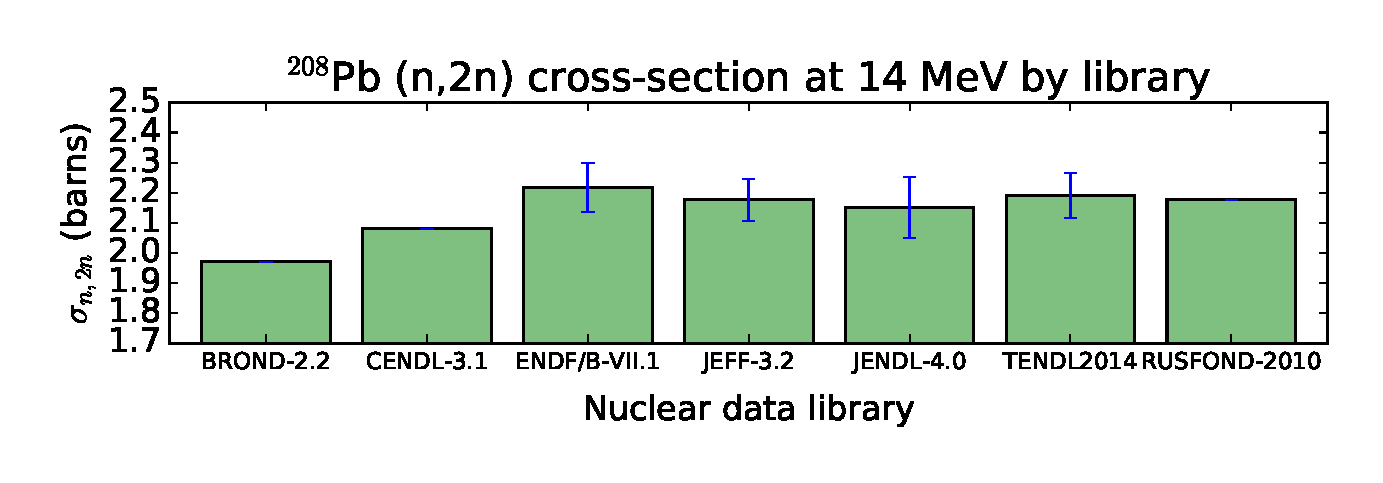
\includegraphics[width=0.47\textwidth]{pb208_n2n_by_lib}
%   \caption{$^{208}$Pb(n,2n)$^{207}$Pb cross-sections at 14MeV with their associated uncertainties for various libraries.}
%   \label{fig:lead_by_library}
% \end{figure}

% Read through section, decide on underlying topics
% Generate sub headings 
% Find papers
% Summarise and write

% HEADINGS
% Uncertainty propagation (see Michael Rising)
%   ? Conventional ?
%   Total Monte Carlo
% Uncertainty in fusion relevant nuclear data
%   Example - DT cross-section?
%   Example - Be multiplicity? O-16 scatter?
%   Example - Lead multiplicity
% END HEADINGS

\FloatBarrier
\subsection{Uncertainty propagation}
% Rising pg 90, ref 83,84
Those in the nuclear engineering field who use nuclear data (ND) are concerned with how `integral' quantities such as heating rates, neutron fluences, TBRs, etc. are impacted by ND uncertainties. To estimate this, one must `propagate' the uncertainty from data to integral quantities. The main approaches are perturbation theory / sensitivity analysis and sampling methods. Perturbatory approaches were developed first and applied with great effect to fission reactor systems. Sampling methods only became available with the increases in computing power achieved in the 21\textsuperscript{st} century. The basics of the methods and the merits and demerits of each are described below.

\FloatBarrier
\subsubsection{Perturbation and sensitivity}
\label{subsubsec:pert}
Perturbation theory is widely applied in many branches of the sciences, and generally consists of substituting an unsoluble equation for a related, soluble one plus some perturbatory series of terms. These increasing order terms have less and less impact on the result and the series is truncated at some point. 

Work on applying this approach to reactor physics problems was undertaken by Wigner on the first nuclear pile \cite{Rising2012}. A more sophisticated framework was developed by Gandini, the Generalised Perturbation Theory (GPT) \cite{Gandini1967} and subsequently into the Equivalent Generalised Perturbation Theory (EGPT) \cite{Gandini1986}. These efforts require obtaining the forward and adjoint solutions to the Boltzmann transport equation such that one can identify the magnitude of responses to any input perturbation. This means GPT and EGPT naturally lend themselves to deterministic methods for radiation transport, where full solutions to the Boltzmann equation are obtained, rather than a subsection of its phase space sampled (as in stochastic methods). This was overcome relatively recently for fission with codes like TSUNAMI-3D by Rearden, which can calculate uncertainties in $k_{\mathrm{eff}}$ with deterministic or Monte Carlo methods \cite{Rearden2004}. An alternative method, not specific to fission problems, is to couple a radiation transport code such as MCNP \cite{Goorley2012} with the SUSD or SUS-3D codes \cite{Kodeli2001}. MCNP is used with perturbed cross-sections to determine how sensitive, $S$, a response parameter, $R$, is to changes, $\delta \sigma_{g}$, in a cross-section group, $\sigma_{g}$, as shown in equation~\ref{eq:sensitivity}. 

\begin{equation}
  \label{eq:sensitivity}
  S = \frac{(\delta R)/R}{(\delta \sigma_{g}) / \sigma_{g}}
\end{equation}

SUS-3D can be used to combine processed covariance information with these sensitivity profiles to determine the uncertainty in various response parameters. Further detail on perturbation theory applied to radiation transport systems can be found in \cite{Sabouri2013}.

A disadvantage of perturbation theory methods is that they embody a linear relationship between input and output uncertainty (see equation~\ref{eq:sensitivity}). Also, covariance matrices are based on normally distributed uncertainties, whether or not this is in reality the case. The method is very much dependent on the quality and comprehensiveness of covariance matrices available. Very large and difficult to compile covariances matrices are required to record the potential correlations between all open reaction channels. 

\nomenclature[z]{GPT}{Generalised Perturbation Theory} 
\nomenclature[z]{EGPT}{Equivalent Generalised Perturbation Theory} 
\nomenclature[z]{TSUNAMI-3D}{Tools for Sensitivty and Uncertainty Analysis Methodology Implementation in three Dimensions}

\FloatBarrier
\subsubsection{Total Monte Carlo}
\label{subsubsec:tmc}
Koning and Rochman developed a new, integrated method of uncertainty propagation in the late 2000s \cite{Koning2008}. This approach, known as Total Monte Carlo (TMC), relies on repeated sampling of varied nuclear data. Whichever problem is being investigated is simulated multiple times with different data, building a distribution of outcomes. It is a fundamentally different method to the sensitivity / perturbation approach. 

The foundation is a reliable methodology for generating nuclear interaction data. The software package T6 \cite{Koning2005} collects together various frameworks for analysing nuclear interactions such as direct reaction, pre-equilibrium and fission models. 

Using these tools and a set of input parameters, reaction likelihoods and outcomes can be simulated for a variety of incident particles: neutron, photons, protons, deuterons, tritons helions and alpha-particles and for a range of energies from $10^{-5}\mathrm{eV}$ to $200\mathrm{MeV}$. The theoretical models require parameters which may be directly experimentally measured, or are estimated through fitting to other, robust experimental data such as total cross-sections, $\sigma_{t}$. The RIPL-3 nuclear parameter database \cite{Capote2009} contains reference values and confidence estimates for many of these parameters. These and other sources have been assimilated and parsed to provide default values for TALYS, with variances. 

\begin{figure}
  \centering
  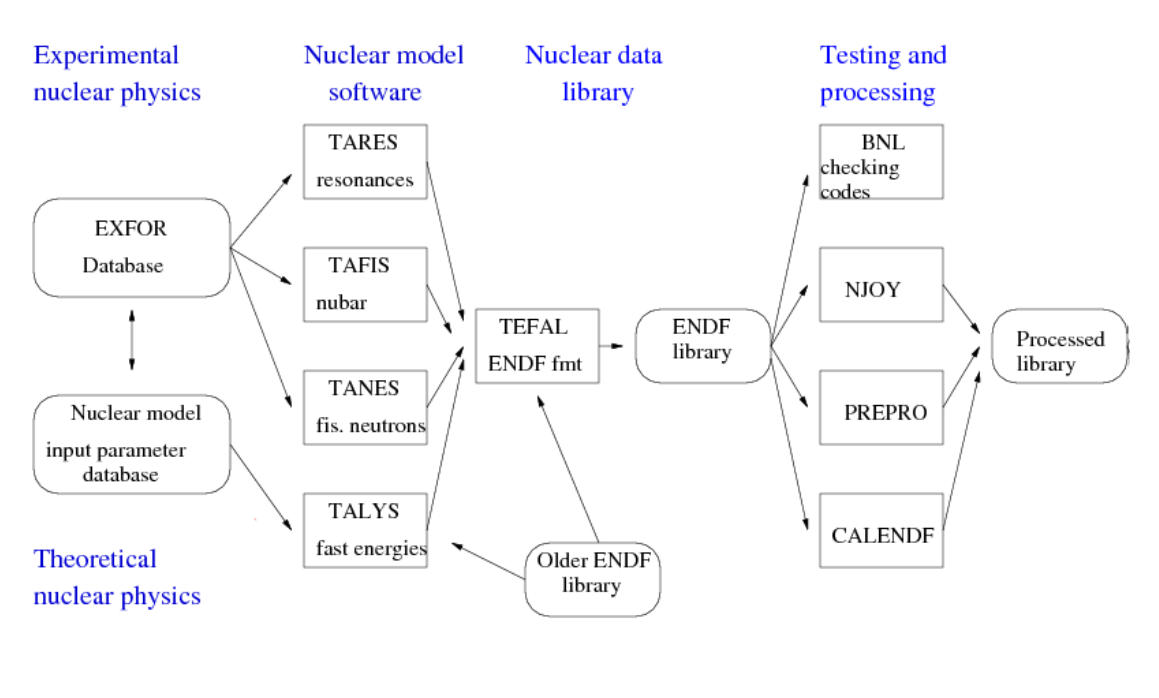
\includegraphics[width=\textwidth]{t6_flow.png}
  \caption[Nuclear data generation in T6 package.]{Nuclear data generation flowchart for the T6 software package. Figure from \cite{Koning2013}.}
  \label{fig:t6_overview}
\end{figure}

A set of nuclear parameters, $\vec{A} = [A_{1},\ldots,A_{n}]$, are used as input to T6 to generate a complete ND library, with full cross-section, resonance, angular distribution, double-differential distribution, covariance, etc. information. These data are self-consistent. An example of this behaviour is where a total cross-section is well understood, it is to be expected that a reduction in one reaction channel cross-section, say elastic scattering, would correspond with an increase in another open reaction channel. This correlation is not reproduced with simple adjustment or perturbatory approaches to uncertainty propagation. Once the ND have been generated they are processed and formatted to the ENDF standard with the TEFAL component of the T6 package, permitting use by all ENDF compliant codes \cite{Koning2012}. The ND generation process is shown as figure~\ref{fig:t6_overview}.

Using the above nuclear physics parameter database and models, it is possible to repeat the nuclear data generation process to create a `library of libraries', implicitly containing amongst their variance the uncertainty in the underlying nuclear physics parameters, $\vec{A}$. This data is now used as input to whichever nuclear system is to be simulated. Numerous simulations are launched, each picking a new set of input data, an evaluation from the library of libraries. Whichever reaction rates or spectral quantities can be tallied for inspection and subsequent analysis. Call the quantity of interest $q$. As the number of simulations, $n$, increases, any histogram of the values of $\vec{q} = [q_{1},\ldots,q_{n}]$ will converge to a probability distribution function of the most likely value and its associated uncertainty, $\sigma_{observed}$. 

In an ideal case, this observed uncertainty would all be due to the variations in nuclear data, as in equation~\ref{eq:det_variance_sum}.

\begin{equation}
  \label{eq:det_variance_sum}
  \sigma_{observed}^{2} = \sigma_{A}^{2} 
\end{equation}

Indeed this is the case for deterministic methods. With Monte Carlo methods however, answers are inherently uncertain. Rather than solving an equation to find the exact flux and associated reaction rates at every point, the system behaviour is sampled by virtual particles (see section~\ref{sec:radiation_transport} in chapter~\ref{chap:introduction}). Monte Carlo methods depend on the Law of Large Numbers (LLN), using a large number of simulated particles to converge on some mean behaviour. Far fewer particles populate the simulation than the real system. Short of an infinite number of `source' particles, there is always an associated uncertainty. 

Therefore, in this work the observed uncertainty, $\sigma_{observed,i}$ from a simulation $i$ is composed of two components: uncertainty from the simulation method, the standard deviation $\sigma_{stat.,i}$ and uncertainty from the nuclear data, the standard deviation being $\sigma_{A,i}$. So long as these are independent, their variances sum to give the total variance, as in equation~\ref{eq:variance_sum}.

\begin{equation}
  \label{eq:variance_sum}
  \sigma_{observed,i}^{2} = \sigma_{A,i}^{2} + \sigma_{stat.,i}^{2}
\end{equation}

Assembling a histogram of the simulated values, $\vec{q}$, approximates the underlying PDF of the quantity, $q$ of interest. We can modify equation~\ref{eq:variance_sum} from the single simulation case to extract information on the nuclear data uncertainty contained within the PDF of all simulations. The average statistical standard deviation, $\overline{\sigma}_{stat.}^{2}$, shown in equation~\ref{eq:average_stat} is simply the mean value from all $n$ simulations. Substituting this for $\sigma_{stat.,i}$ we have equation~\ref{eq:average_variance_sum}. 

\begin{equation}
  \label{eq:average_stat}
  \overline{\sigma}_{stat.}^{2} = \frac{1}{n} \sum^{n}_{i=1}\sigma^{2}_{stat.,i}
\end{equation}

\begin{equation}
  \label{eq:average_variance_sum}
  \sigma_{observed}^{2} \approx \sigma_{A}^{2} + \overline{\sigma}_{stat.}^{2}
\end{equation}

If the variance due to nuclear data, $\sigma_{A}^{2}$, is to be known, one must either enforce $\overline{\sigma}_{stat.}^{2} = 0$, or otherwise find the difference between the observed and `statistical' simulation variance. 

In terms of determining this statistical simulation uncertainty, Monte Carlo codes provide an estimate of $\sigma_{stat.,i}$. Comparing this uncertainty amongst differing values of $q$ can be achieved by normalising by $q$. The Relative Standard Deviation (RSD)\footnote{Also known as the Fractional Standard Deviation (FSD)}, $R$, is given below as equation~\ref{eq:rsd} and its functional dependence on particle count as equation~\ref{eq:rsd_m}.

\begin{equation}
  \label{eq:rsd}
  R = \frac{\sigma_{stat.}}{q}
\end{equation}

\begin{equation}
  \label{eq:rsd_m}
  R \propto \frac{1}{\sqrt{m}}
\end{equation}

Where $q$ is the reported quantity mean value and $m$ is the simulation particle population count. Keeping $R$ to an arbitrarily small value, say <0.005, allows us to ignore the $\overline{\sigma}_{stat.}^{2}$ term in equation~\ref{eq:average_variance_sum} \cite{Rochman2014a}.

If only one nuclear parameter, $A_{i}$, is varied then the nuclear data uncertainty, $\sigma_{A}$ is wholly attributable to that parameter. Similarly, if only one nuclide has its nuclear parameters and hence interaction data varied, $\sigma_{A}$ represents uncertainty on $q$ from that nuclide alone. When more parameters are varied for more nuclides, the uncertainty is an ensemble of their variation. 

\nomenclature[z]{RSD}{Relative Standard Deviation}
\nomenclature[z]{LLN}{Law of Large Numbers}

The general TMC process is diagrammatically outlined in figure~\ref{fig:tmc_overview}. Compared to other methods, this approach has a variety of benefits. One advantage of this system is that one relates uncertainty in the earliest possible parameters, say the real volume potential or imaginary surface potential of the optical model to the integral quantities of most interest to end-users such as TBR or nuclear heating in a fusion context. This allows future targeting of nuclear physics research--where are resources best allocated to reduce system uncertainties? This is the idea represented by the sensitivity feedback loop in figure~\ref{fig:tmc_overview}. Of course, this methodology does not have to only vary nuclear physics parameters, one can choose to vary parameters in the simulation model, or even methodology, to determine their contribution to uncertainty. Engineering parameters, such as component dimensions, operating temperatures, nuclide atomic densities, etc. can be varied to see how uncertainty on them effects quantities of interest.

\begin{figure}
%  \figuretitle{}
  \centering
  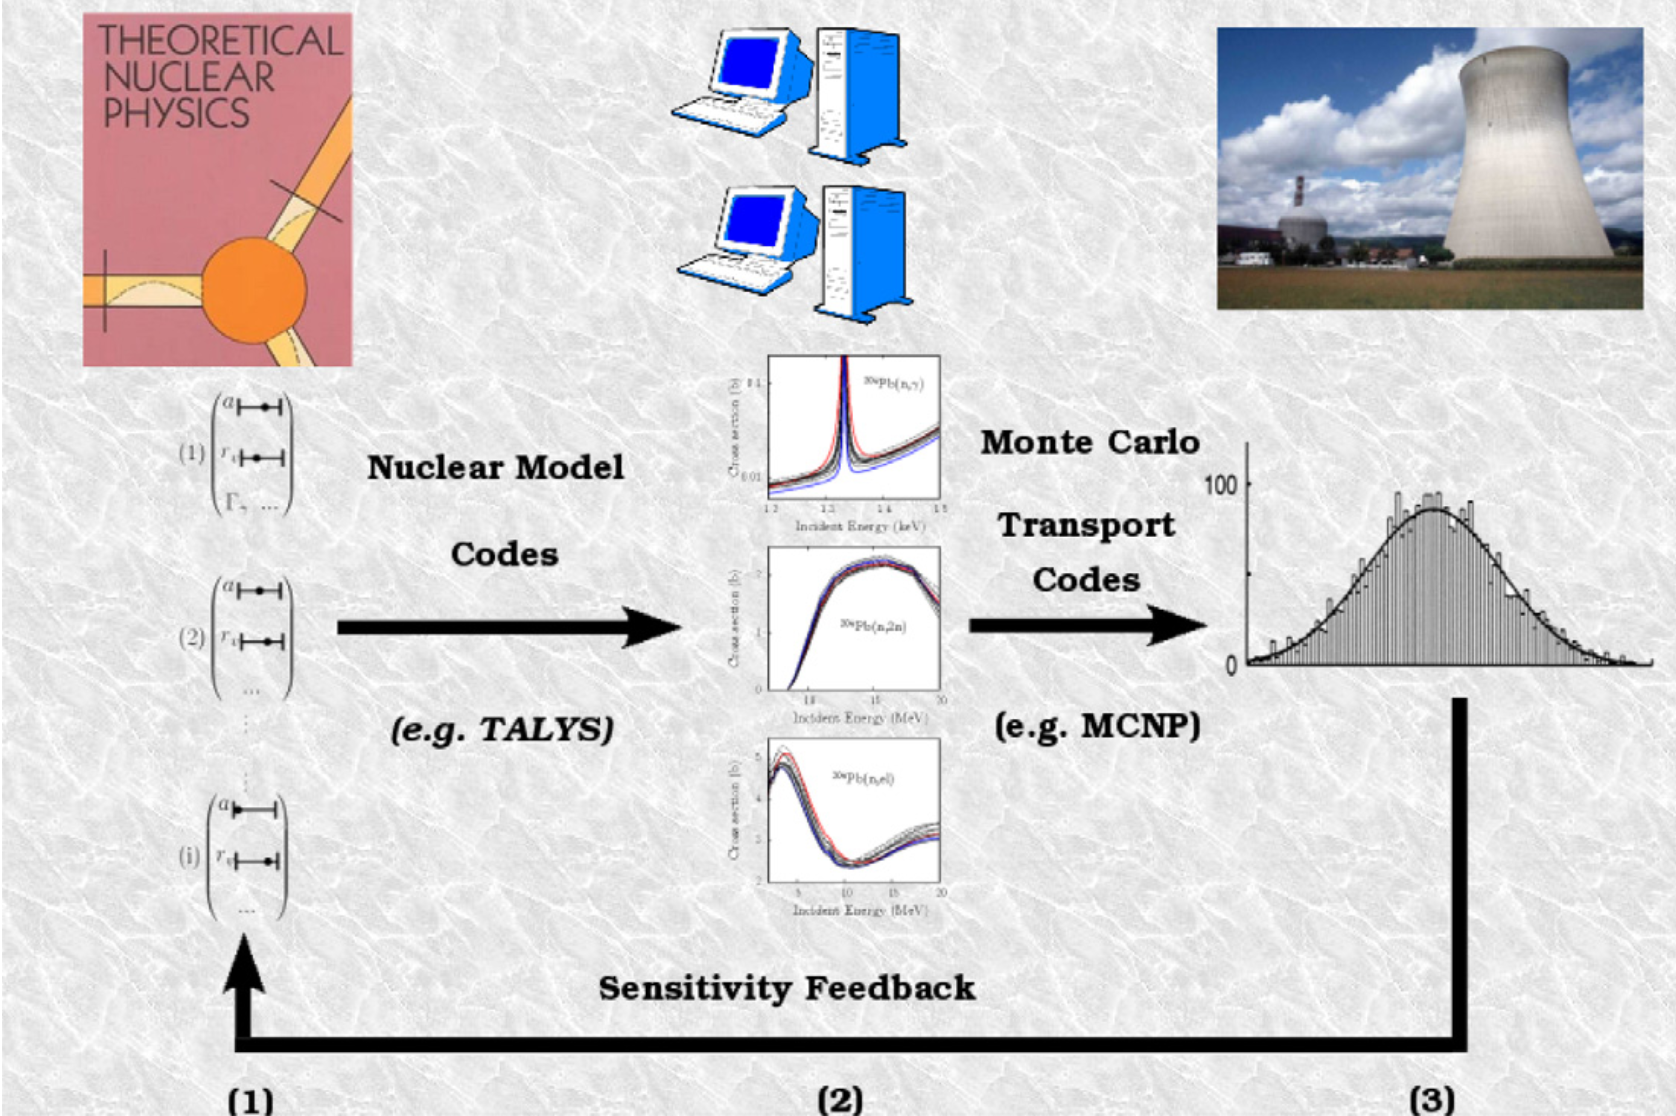
\includegraphics[width=0.8\textwidth]{tmc_overview.png}
  \caption[Total Monte Carlo process schematic.]{Schematic overview of the TMC process. 1) Uncertainties in fundamental nuclear parameters estimated. 2) Many sets of ND generated with T6 software, sampling from fundamental parameters. 3) Nuclear system is simulated many times with generated ND, value of observable is added to PDF, eventually converging on an observable with a mean value and characteristic distribution. Figure from \cite{Koning2008}.}
  \label{fig:tmc_overview}
\end{figure}

\FloatBarrier
\subsubsection{Comparison of methods}
Sections \ref{subsubsec:pert} and \ref{subsubsec:tmc} have discussed the methods of two uncertainty propagation schemes. It is worth noting the advantages and disadvantages of each, drawing some comparisons between them to elucidate where each method might be most appropriate.

The perturbation method, using covariance information and sensitivity profiles, has much experience associated with it. It has been used to estimate uncertainties for $k_\mathrm{eff}$ and other important parameters in fission reactor physics for several decades. By contrast, whilst the idea of repeatedly simulating a system with different inputs is not new, the integrated TMC methodology, with a sophisticated ND generation package, is novel. Published in 2008, it has seen substantially less use in industry than perturbatory approaches. The nuclear industry is often slow to adopt new technology as there can be a significant volume of work required to validate results, especially where their application is safety-critical. Studies in a variety of applications have sought to benchmark and demonstrate TMC, bringing it into wider use \cite{Koning2008}\cite{Rochman2010}\cite{Sjostrand2017}\cite{Koning2012}\cite{Alhassan2013}\cite{Alhassan2014}\cite{Rochman2011a}. 

Assuming appropriate nuclear data is already available, the slowest component of either method is radiation transport by some Monte Carlo code. Combining covariance information with sensitivity profiles, or parsing results from multiple TMC simulations to assemble a PDF of some target quantity, $q$, is of minor computational burden. If the time taken for a single simulation is $T$ time units, then TMC will take $n \times T$ where convergence on some $q$ and its $\overline{\sigma}_{observed}$ typically takes $n \geq 500$ simulations to sufficiently sample input uncertainties \cite{Rochman2014a}. This factor of several hundred slowdown is clearly a burden for many analyses, especially those requiring many billions of source particles such as full-core fission reactor simulations, shielding analyses or similar. 

In the past 3 or 4 years, progress has been made in reducing the TMC time penalty. If a single calculation requires $m$ particles for convergence, so-called `Fast TMC' uses $m/n$ particles in each of the $n$ simulations. This dedicates fewer particle histories to each change in nuclear data, exploring the $A$ parameter-space more quickly, but with a larger $\sigma_{stat.}$ for each simulation. \citeauthor{Rochman2014a} indicate that ensuring the inequality $\frac{\sigma_{stat.}}{\sigma_{observed}} \leq 0.5$ holds for each simulation, equation~\ref{eq:average_variance_sum} is still valid and the scheme still computes approximately the same uncertainties as $n$ runs each with $m$ particles. This is in contrast to traditional TMC where the rule of thumb is $\frac{\sigma_{stat.}}{\sigma_{observed}} \leq 0.05$.

Perturbatory methods require covariance matrices, but often only covariance information for certain phenomena are readily available. Along with cross-sections and resonance parameters there are angular distributions of scattered and emitted particles, double-differential distributions, $\overline{\nu}$ (average neutron yield from a fission event), etc. Evaluations vary in their completeness. As TMC calculates and varies a full complement of nuclear data with its set of nuclear models, it can claim to have a more comprehensive estimate of the true uncertainty. While perturbations to generate sensitivity profiles are for a single cross-section group value (for example), TMC varies parameters at an earlier step, as a fundamental parameter for the behaviour of the nucleus. Because of this, when a parameter is varied in the TMC approach, it in turns varies all correlated phenomena. Other areas where the TMC scheme embodies a more complex approach are the assumed linearity of the perturbation method, along with the inability of perturbation methods to accommodate non-Gaussian observable distributions. Despite these advantages, the TMC method has attracted certain criticisms. It can be argued that the all-important nuclear parameter distributions have not been rigorously estimated from experimental data \cite{Helgesson2017}. Both \citeauthor{Capote2010} and \citeauthor{Rising2012} note the arbitrariness of some parameter distributions. Recently, work has been undertaken to implement Bayes' theorem through the assignment of weights to generated ND \cite{Koning2015a}, based on experimental data and automatically generated covariance files \cite{Helgesson2017}.

% ENDF-6 does not support covariances for some kinds of data, such as double-differential data \cite{ENDF-6}. 

The ease of application of the two methods is varied. While TMC is conceptually easy to understand and incorporates many advantageous features, there are limitations in its application currently, such the failure of TALYS to correctly predict the behaviour of light nuclides (the cut-off being A=12) \cite{Rochman2011}. For perturbation methods, the paucity of covariance information is a problem for some calculations (principally those outside the thermal fission realm). 

\FloatBarrier
\subsection{Uncertainty in fusion relevant data}
There are many nuclides of importance in nuclear fusion studies whose behaviour are not known to sufficient accuracy \cite{Forrest2011}. Nuclear technology development programmes for ITER \cite{Batistoni2008} and DEMO \cite{Abdou2015} have both identified the need for more widespread uncertainty estimates and more accurate nuclear data evaluations to reduce uncertainties. \citeauthor{Batistoni2008} cites conservative uncertainties for neutron fluence at the ITER pressure vessel ($\pm 15\%$) and superconducting Toroidal Field (TF) coil magnets ($\pm 30\%$) due to nuclear data uncertainties. 

An improved uncertainty treatment has been advocated for tritium breeding since the early days of detailed reactor design \cite{Abdou1986}. \citeauthor{Youssef1986} performed a sensitivity / perturbation analysis on uncertainties in TBR due to ND for early blanket designs finding that ND contributed an uncertainty on TBR of between 2--6\% of the mean value depending on the specific design. 

A variety of different tritium breeding schemes are proposed for reactors. These have either solid (ceramic pebbles) or liquid (molten metal) breeding compounds which may or may not be accompanied by an additional neutron multiplying material. The solid systems have some sort of additional coolant loop, typically employing He or H\textsubscript{2}O. For the liquid metal systems, the breeder also functions as the primary coolant. All systems are likely to have a secondary coolant loop for subsequent electricity generation. \citeauthor{Youssef1986} compared the TBR uncertainty due to ND for several of these systems. He found that Li\textsubscript{2}O ceramic systems typically have a large uncertainty contribution from \textsuperscript{16}O, followed by \textsuperscript{56}Fe and the lithium isotopes (their relative importance depending on the degree of \textsuperscript{6}Li enrichment). Uncertainty in a LiAlO\textsubscript{2} system on the other hand was dominated by uncertainty in \textsuperscript{9}Be multiplicity cross-section data. As such, there were significant differences between similar breeding concepts, which is a frustration when trying to generalise and also underscores the importance of this kind of work. For a Li-Pb, liquid metal system, the TBR uncertainty was dominated by variance in the lead multiplicity cross-sections, the (n,2n) and to a lesser extent (n,3n) reactions.

As well as pure computation, work is available comparing simulation and experimentally determined values for important reaction reaction channels in ceramic (HCPB) tritium breeding systems \cite{Batistoni2007}. Less work has been undertaken to experimentally corroborate simulated nuclear responses in liquid metal blankets. This is not for lack of desire, these lithium-lead blankets are currently in development in tandem with the solid breeders and account for half of the Test Blanket Modules (TBM) to be tested in ITER \cite{Chuyanov2010}. There are good reasons to expect lithium-lead blankets to be yet further developed, reasons including: the greater resource availability (beryllium for ceramic blankets is in limited supply \cite{Bradshaw2011} \cite{Shimwell2014}), the facility for on-load lithium enrichment and thus TBR adjustment \cite{Ihli2008}, higher natural breeding ability \cite{Colling2012} and the comparative ease of extracting bred tritium from a liquid metal vs. porous pebbles. A more thorough discussion on the advantages and disadvantages of the different technologies can be found in \cite{Abdou2015}. Given the above, it is worth investigating the impact of ND uncertainties on LiPb type blankets.

%\nomenclature[z]{HCPB}{Helium Cooled Pebble Bed}
%\nomenclature[z]{HCLL}{Helium Cooled Lithium Lead}
\nomenclature[z]{TBM}{Test Blanket Module}
\nomenclature[z]{TF}{Toroidal Field}

% The other examples seem strange to include if there's not going to be any TMC analysis...
%\subsubsection{Deuterium-Tritium}
%\subsubsection{\textsuperscript{16}O scattering}
%\subsubsection{Lead multiplicity}

As briefly mentioned previously, \citeauthor{Leichtle2011} has undertaken a recent study where nuclear data was adjusted to obtain the sensitivity of TBR in a modern HCLL system (the ITER HCLL TBM) to various nuclear reaction cross-sections \cite{Leichtle2011}. This work identified $^{6}$Li, $^{56}$Fe and the Pb cross-sections as the most important for TBR uncertainty from the a ND perspective. The analysis below looks at variation in lead nuclear data. 

\FloatBarrier
%\subsection{DEMO}
% Should this be here? Perhaps it doesn't need a whole bit...

\FloatBarrier
\section{Method}
This chapter is investigating the propagation of lead nuclear data uncertainties to a corresponding PDF for TBR uncertainty in the DEMO reactor. The following section describes nuclear data selection and sampling, along with radiation transport and data analysis methods for the study.

\subsection{Nuclear data}
\label{subsec:data}
As discussed in section~\ref{subsubsec:tmc}, traditionally cross-section uncertainties are represented as single values for a given energy and reaction channel. There might be an estimate of uncertainty, which is typically given as a 1 $\sigma$, the standard deviation of a Gaussian distribution centred about the quoted mean value. As an example, the $^{208}$Pb(n,2n)$^{207}$Pb neutron multiplication reaction at 14 MeV is shown in table~\ref{tab:lead_by_lib} for a variety of experiments and nuclear data libraries. Experimental results from the EXFOR library are also shown. There are a wide spread of experimental results, for example Arakita and Shunk are relatively low at 1.04 and 1.31 b respectively and with quoted uncertainties of 5.77 and 8.0\% respectively. These values are among the older data experimental data and have been relegated in importance by nuclear evaluators. Modern evaluated data releases tend to agree on a figure of $\sigma_{n,2n}(14\ \mathrm{MeV}) \approx 2.1$ barns. It would appear that the experiments of Simakov and Frehaut along with model calculations have been favoured of to produce the data contained within contemporary evaluated nuclear data libraries. Data shown in table~\ref{tab:lead_by_lib} are also shown graphically in figure~\ref{fig:tendl_lead} along with the 300 TENDL files used for this work.

\begin{table}[H]
  \footnotesize
  \centering
  \begin{tabularx}{\textwidth}{XXXX}
    \toprule
    Source & Energy [MeV] & $\sigma_{n,2n}$ [b] & $\pm\%\Delta\sigma_{n,2n}$ \\
    \midrule
    Experimental data &      &      &    \\
    \midrule
    Ngoc & 14.6 & 1.27 & 7.61 \\
    Simakov & 14.1 & 2.38 & 5.88 \\
    Anders & 14.6 & 1.36 & 4.98 \\
    Arakita & 14.2 & 1.04 & 5.77 \\
    Frehaut & 13.8 & 1.96 & 8.11 \\
    Frehaut & 14.3 & 1.94 & 8.36 \\
    Frehaut & 14.8 & 1.97 & 8.52 \\
    Salaita & 14.8 & 1.31 & 8.85 \\
    Shunk & 14.0 & 1.31 & 8.00 \\
    Prasad & 14.8 & 0.99 & 12.12 \\
    Garg & 14.7 & 1.09 & 6.78 \\
    Glagolev & 14.7 & 1.70 & 17.65 \\
    Amemiya & 14.8 & 1.22 & 8.20 \\
    \midrule
    Evaluated data &      &      &    \\
    \midrule
    BROND 3.1 & 14.0 & 2.09 & - \\
    CENDL 3.1 & 14.0 & 2.08 & - \\
    ENDF/B-VII.1 & 14.0 & 2.22 & 8.15 \\
    JEFF 3.2 & 14.0 & 2.18 & 7.0 \\
    JENDL 4.0 & 14.0 & 2.15 & 10.1 \\
    TENDL 2015 & 14.0 & 2.19 & 7.4 \\
    RUSFOND 2010 & 14.0 & 2.18 & - \\
    \bottomrule
  \end{tabularx}
  \caption[Cross-section and uncertainty data for the $^{208}$Pb(n,2n)$^{207}$Pb reaction.]{Cross-section values for the n,2n reaction channel, $\sigma_{n,2n}$ on $^{208}$Pb, around 14 MeV for various experiments and libraries. The experimental results were retrieved from the online EXFOR database \cite{exfor2017}. The ENDF utility code Inter \cite{Dunford2002} was used to extract the values for each library. The uncertainties, $\Delta\sigma_{n,2n}$ are presented as percentages above and below the reported value.}
  \label{tab:lead_by_lib}
\end{table}

% \begin{figure}[H]
%   \centering
% %  \figuretitle{}
%   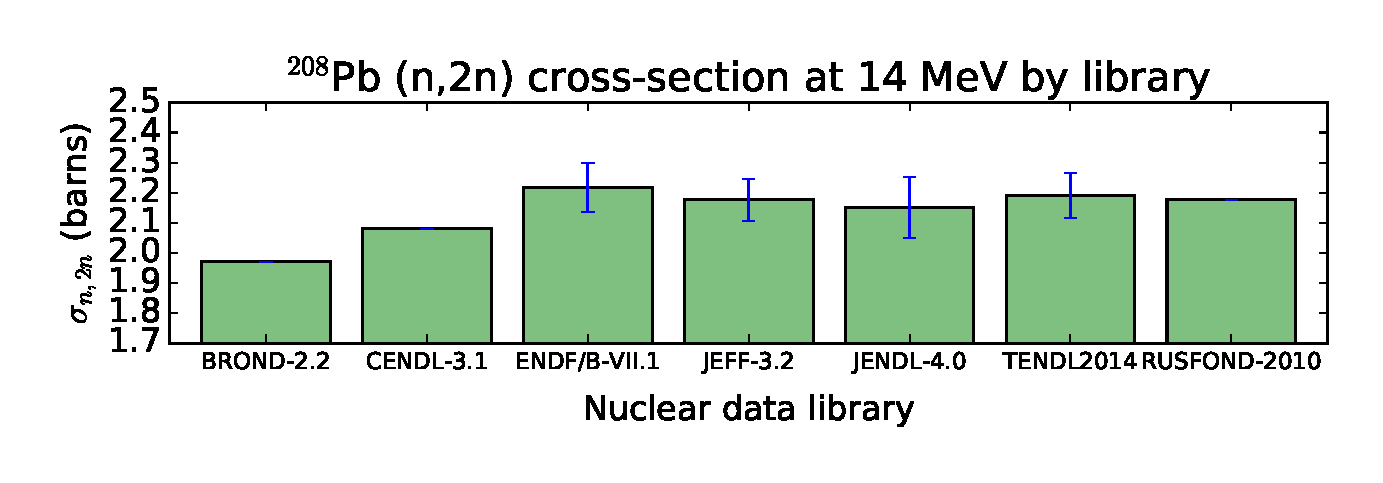
\includegraphics[width=\textwidth]{pb208_n2n_by_lib}
%   \caption{Comparison of (n,2n) cross-section values in major ND libraries for the most abundant lead isotope, $^{208}$Pb. Uncertainties are shown where available.}
%   \label{fig:lead_by_lib}
% \end{figure}

This study used the TENDL-2015 library. It is a comprehensive, general-purpose nuclear data library which contains data on interactions between 7 projectiles and over 2,800 target nuclides. As described above, the library is produced by a suite of codes known as T6 and an adherence to a strict methodology of reproducability \cite{Rochman2016}. It uses the TALYS nuclear reaction code to model high-energy reactions, with TARES handling the lower energy, resonant region. The inputs are fundamental parameters, including data from the RIPL-3 database \cite{Capote2009}, each with their own probability distributions that reflect their uncertainties. The TENDL-2015 release contains `average' or best-guess evaluations, but also a collection of `random' files, those generated using the sampling method. These have been pre-generated by the TENDL team. Comprehensive information concerning the input parameters and plots of the ND are available online \cite{TENDL2015}.

It is instructive to inspect the nuclear data used as input for this TMC simulation. The sampled nuclear data files were downloaded in both ACE (293K) and ENDF format from the TENDL-2015 website \cite{TENDL2015}. Figure~\ref{fig:tendl_lead} shows the (n,2n) cross-sections as a function of energy for $^{208}$Pb. Cross-sections from a given file at a certain energy are shown as grey circles. The mean value of the random files and a standard deviation is also shown, along with available EXFOR data. The shape of this endothermic multiplication reaction is visible, with an energy threshold of 7.36 MeV. The cross-section rises to approximately 2 b in the 14 MeV fusion neutron energy range before falling away at higher energies--here the n,3n reaction becomes more probable. No experimental data is available from the EXFOR database beyond 14.8 MeV. This lack of higher energy information means constraining model parameters for T6 data generation is more difficult and so the uncertainties here are larger.

% \begin{figure}
% %  \figuretitle{}
%   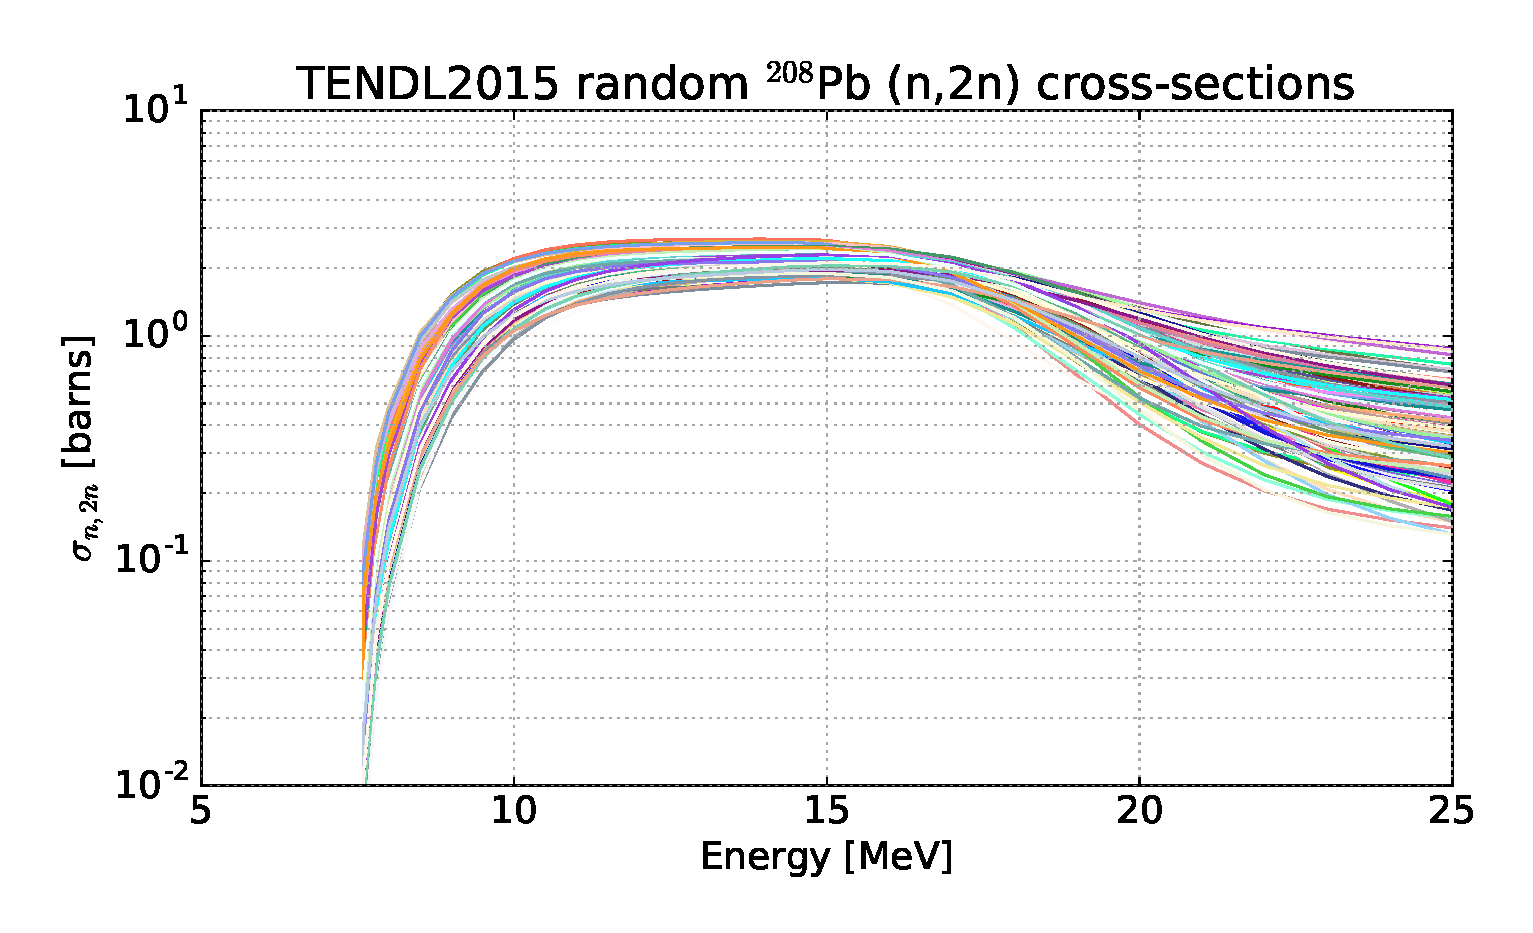
\includegraphics[width=0.48\textwidth]{pb208_tendl_n2n}
%   \caption{Shown here are 300 `random' TENDL2015 n,2n cross-sections as a function of energy for the most abundant lead isotope, $^{208}$Pb.}
%   \label{fig:tendl_lead}
% \end{figure}

\begin{figure}[H]
%  \figuretitle{}
  \centering
  \makebox[\textwidth][c]{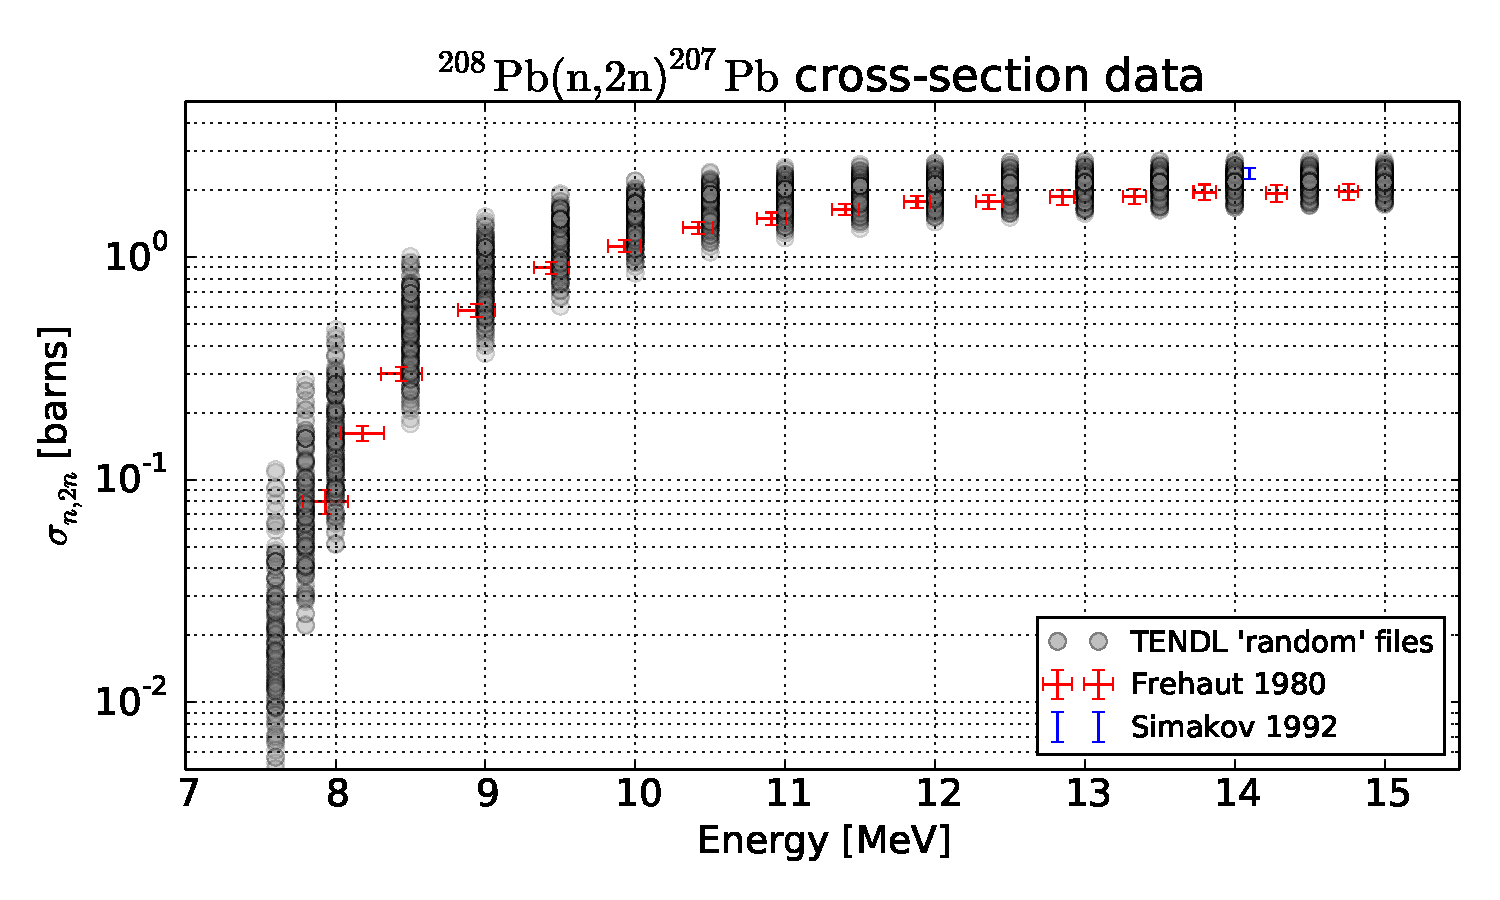
\includegraphics[width=1.1\textwidth]{pb208_n2n_tendl_exfor}}
  \caption[Cross-section and uncertainty data for the $^{208}$Pb(n,2n)$^{207}$Pb reaction.]{Shown here are $^{208}$Pb(n,2n)$^{207}$Pb cross-sections as a function of energy. The plot shows the TENDL `random' data extracted from processed ACE files. Additionally, the few available experimental results in EXFOR are plotted for comparison. The relative paucity of experimental data is one reason for the relatively large uncertainty on this particular reaction channel.}
  \label{fig:tendl_lead}
\end{figure}

In an unmoderated fusion neutron spectrum the dominant reaction channels for Pb are neutron multiplication (n,2n) and elastic scattering, at approximately 2 and 3 barns respectively. The ENDF utility code Inter was used to extract cross-section values at a given energy from the ENDF files. The resulting distributions and correlations were plotted as figures \ref{fig:tendl_n2n}, \ref{fig:tendl_nel} \& \ref{fig:pb_el_n2n_corr}. Figures \ref{fig:tendl_n2n} and \ref{fig:tendl_nel} were examined for their first 3 statistical moments. 

\begin{table}[H]
  \footnotesize
  \centering 
  \begin{tabular}{llll}
    \toprule
    Nuclide & Mean, $\mu$ [b] & RSD, $\frac{\sigma}{\mu}$ & Skewness \\
    \midrule
    Pb206 & 2.11 & 8.1\% & -0.065 \\
    Pb207 & 2.12 & 10.7\% & -0.868 \\
    Pb208 & 2.17 & 9.7\% & -0.120 \\
    \bottomrule
  \end{tabular}
  \caption[Statistical moments of $^{208}$Pb(n,2n)$^{207}$Pb data in TENDL2015.]{TENDL2015 `random' Pb n,2n neutron multiplicity channel cross-section distribution statistics, also shown in figure~\ref{fig:tendl_n2n}.}
  \label{table:n2n}
\end{table}

Figure~\ref{fig:tendl_n2n} and table~\ref{table:n2n} show the distributions of TENDL-2015 cross-sections for (n,2n) at 14 MeV. Lower values for $\sigma_{n,2n}$ will reduce the neutron multiplication of the blanket and, other quantities being equal, result in a reduced total neutron flux and therefore a lower TBR. The first two moments of each distribution in figure~\ref{fig:tendl_n2n} were analysed for convergence testing. A normalised measure of the standard deviation, the relative standard deviation, $R(n) = \frac{\sigma(n)}{\mu(n)}$, where $\sigma(n) = \sqrt{\frac{\sum_{i=0}^{n}(x_{i}-\mu_{i})^{2}}{n-1}}$ and $\mu(n) = \frac{\sum_{i=0}^{n}x_{i}}{n}$ was plotted as a function of sample size. $R(n)$ converges for $n \approx 150$ for both $^{206}$Pb and $^{208}$Pb at 8.1\% and 9.7\% respectively. For $^{207}$Pb, $R(300)=10.7\%$, but this figure is not completely converged, with some step changes in $R$ due to extreme $\sigma_{n,2n}$ cross-sections from the low-value tail. Ideally more data would be available for this nuclide.

\begin{figure}[H]
%  \figuretitle{}
	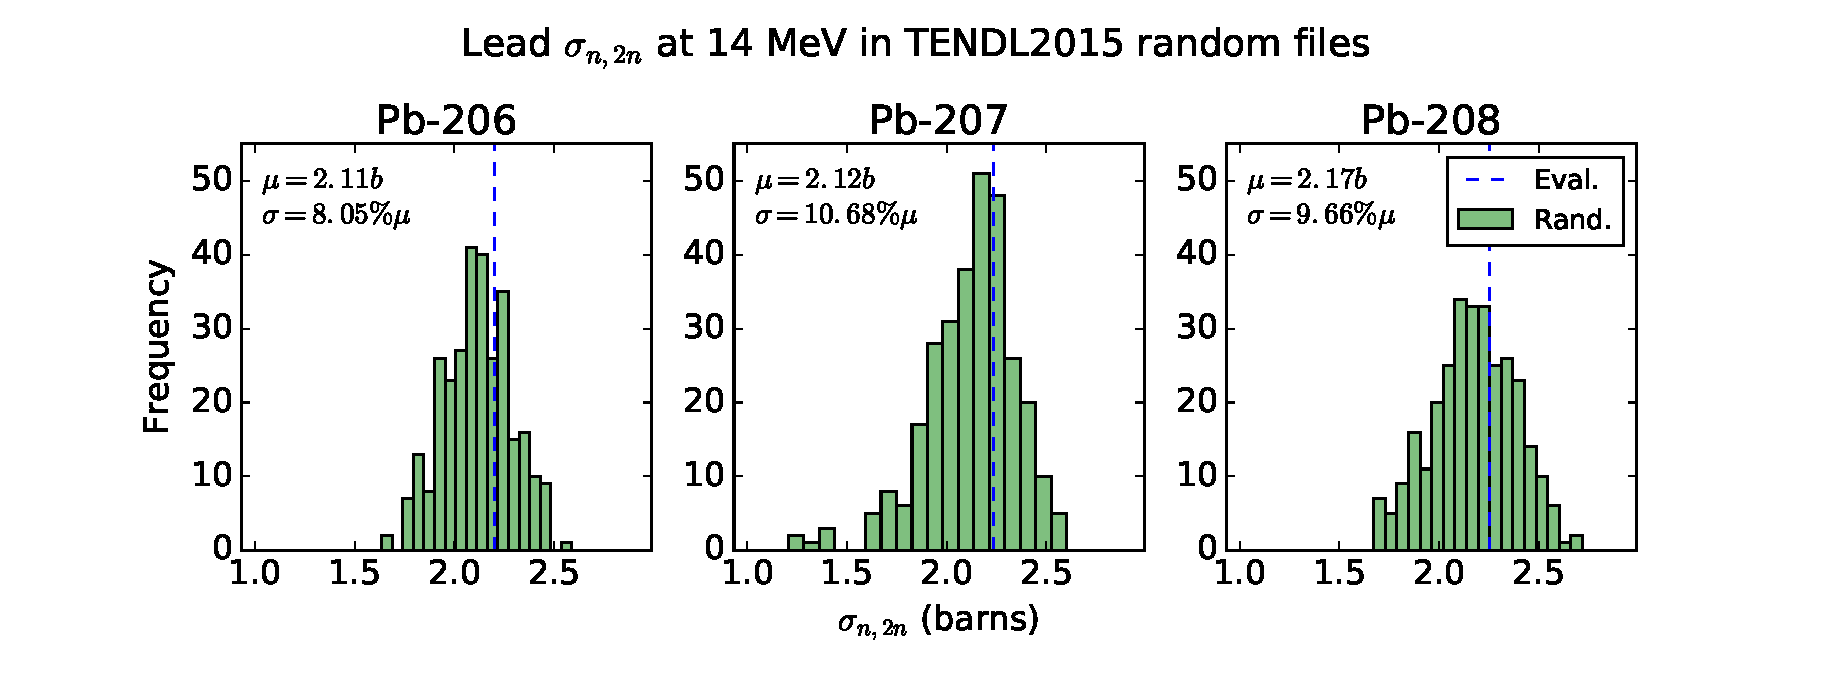
\includegraphics[width=\textwidth]{pb_tendl_n2n_hist}
	\caption[Histograms of $^{208}$Pb(n,2n)$^{207}$Pb data in TENDL2015.]{Shown are histograms of $\sigma_{n,2n}$ at 14 MeV for the three major Pb isotopes. The histogram contains all 300 available files each Pb nuclide. It can be seen that while $^{206,208}$Pb are approximately symmetrical with skewness values close to zero, $^{207}$Pb has a skewness of -0.868 indicating a low-value tail. This may or may not be representative of the underlying distribution.}
	\label{fig:tendl_n2n}
\end{figure}

\begin{table}[H]
  \footnotesize
  \centering 
  \begin{tabular}{llll}
    \toprule
    Nuclide & Mean, $\mu$ [b] & RSD, $\frac{\sigma}{\mu}$ & Skewness \\
    \midrule
    Pb206 & 2.84 & 7.5\% & 0.663 \\
    Pb207 & 2.80 & 8.0\% & 0.548 \\
    Pb208 & 2.81 & 8.1\% & 1.185 \\
    \bottomrule
  \end{tabular}
  \caption[Statistical moments of $^{208}$Pb(n,el)$^{208}$Pb data in TENDL2015.]{TENDL2015 `random' Pb elastic scattering cross-section distribution statistics, also shown as figure~\ref{fig:tendl_nel}.}
  \label{table:nel}
\end{table}

\begin{figure}[H]
%  \figuretitle{}
  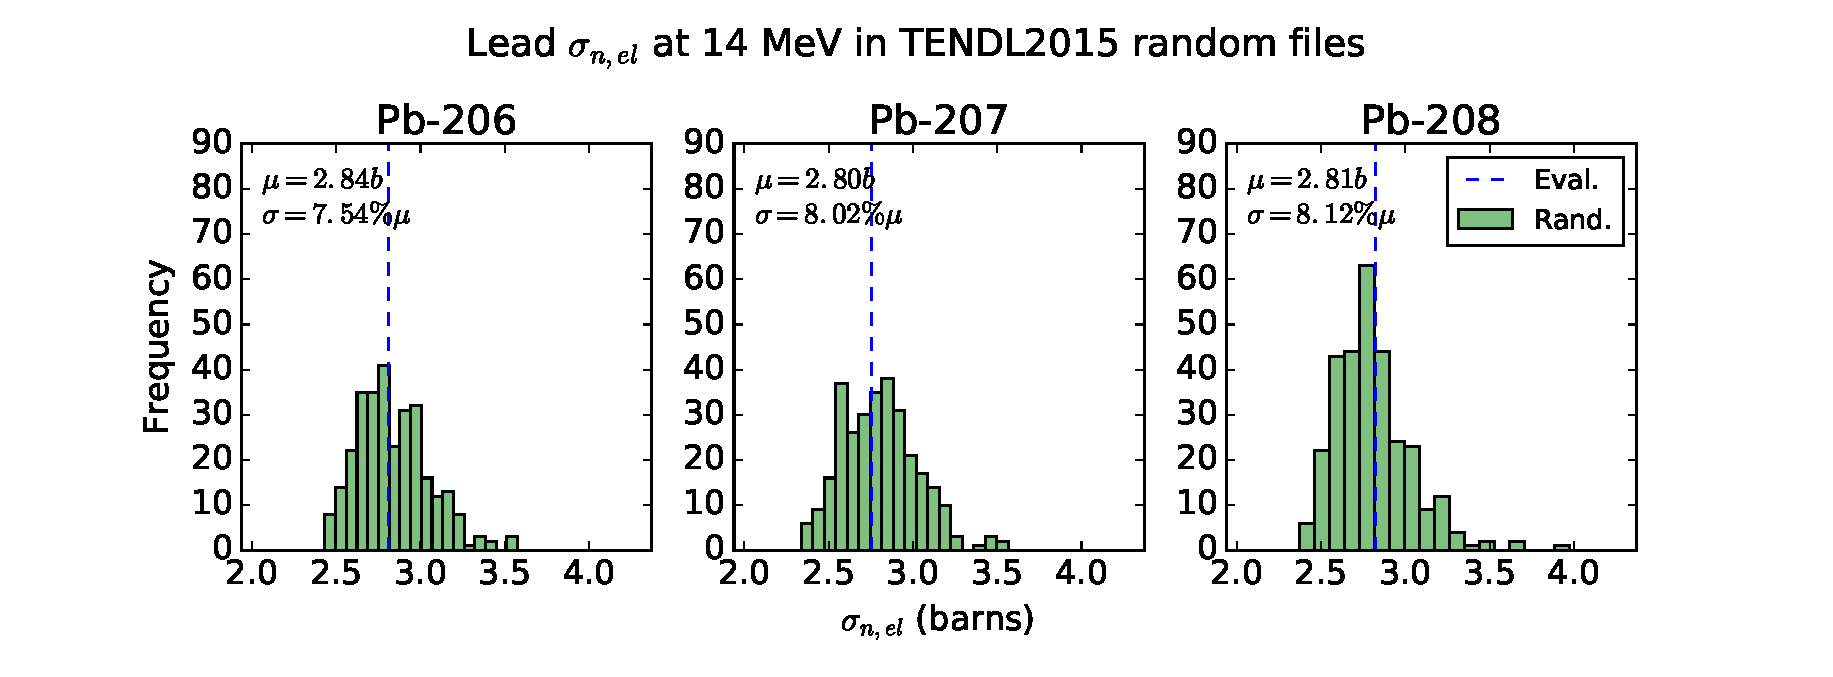
\includegraphics[width=\textwidth]{pb_tendl_nel_hist}
  \caption[Histograms of $^{208}$Pb(n,el)$^{208}$Pb data in TENDL2015.]{The elastic scattering cross-sections for lead at 14MeV are all positively skewed, with $^{208}$Pb having a skewness value of 1.185.}
  \label{fig:tendl_nel}
\end{figure}

The elastic scattering data shown in figure~\ref{fig:tendl_nel} and table~\ref{table:nel} are instead positively skewed, with high value tails for each isotope, with the most pronounced tail being $^{208}$Pb. A greater elastic scattering cross-section will result in an increased likelihood of down-scattering neutrons to lower energies. The softer spectrum will increase triton production in $^{6}$Li as the cross-section increases with decreasing energy, i.e. $\sigma_{n,t}(E) \propto \frac{1}{E}$. However, the elastic scattering cross-section is anti-correlated with the n,2n cross-section in the TENDL data (see figure \ref{fig:pb_el_n2n_corr}). In other words, a high scatter cross-section is typically coupled with a low multiplicity cross-section. This inclusion of cross-channel correlation is one of the key advantages of TMC over more traditional uncertainty propagation (UP) methods. 

% This compensating effect decreases the overall uncertainty where individual perturbations on a single channel would result in an unrealistic, larger uncertainty. 

\begin{figure}[H]
%  \figuretitle{}
	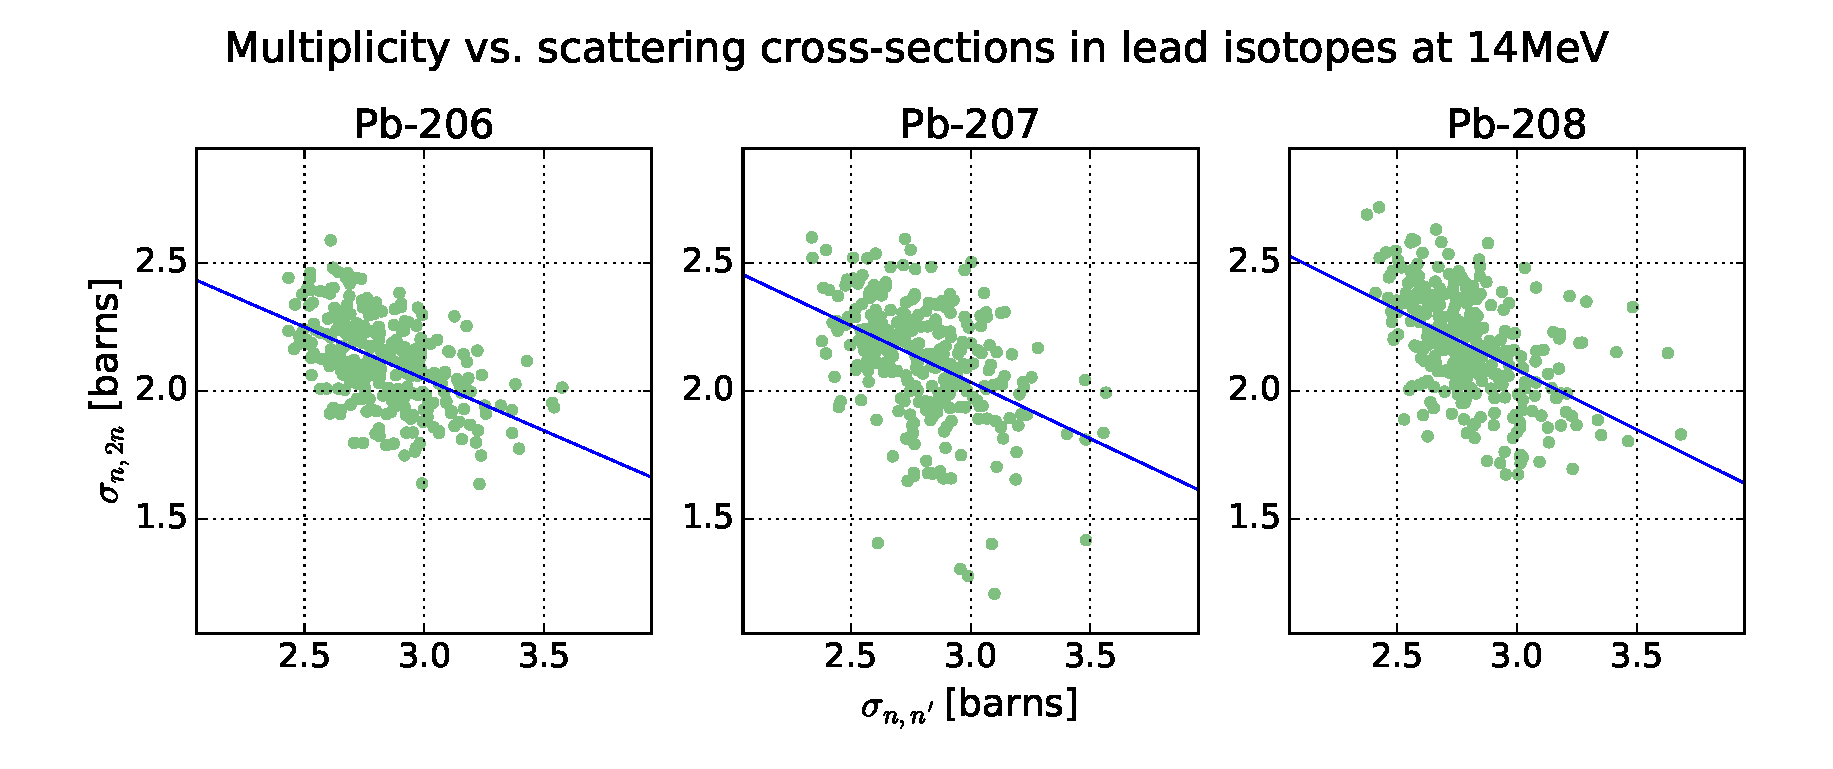
\includegraphics[width=\textwidth]{pb_el_n2n_corr}
  \caption[Correlation between elastic and (n,2n) channels in Pb.]{Shown here are scatter plots of the relationship between the scattering and n,2n cross-sections in the TENDL data. The two channels are clearly anti-correlated. A least squares fit has been applied and the resulting best-fit linear relationship plotted.}
	\label{fig:pb_el_n2n_corr}
\end{figure}

\FloatBarrier
\subsection{Radiation transport}
There exist several variants on the DEMO future fusion reactor concept. It is typically a several GW\textsubscript{th} device, with a major radius, $\mathrm{R}\approx9\mathrm{m}$. Different breeding blanket concepts are the topic of contemporary study and a radiation transport model is typically produced for each one. Of course the nuclear responses within the blanket are of particular interest, but the size and material composition of the blanket also determines the neutron spectra and flux behind them--throughout the rest of the machine.

\begin{figure}[H]
  \centering
	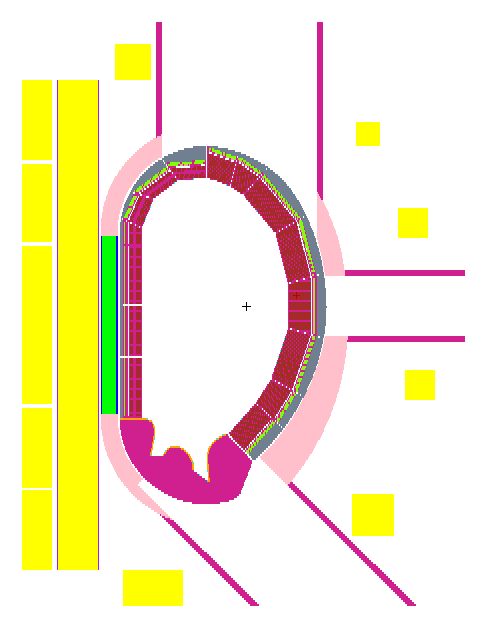
\includegraphics[width=0.5\textwidth]{demo_mcnp}
	\caption[Poloidal slice through DEMO HCLL MCNP model.]{A poloidal slice through the 2014 DEMO HCLL radiation transport model used for this study. Magnets are marked in yellow, the divertor is fuscia and the blanket in red. The blanket sectors are constructed using the MCNP `universe' feature for repeating geometry and do not conform perfectly to the vacuum vessel shape. The three large voids above, below and to the right of the plasma chamber are access ports--extraction routes for blanket and divertor sectors in need of replacement. As noted previously, the distance from the left of this figure to the centre of the plasma chamber is approximately 9m.}
	\label{fig:demo_mcnp}
\end{figure}

An 11.25\degree \ toroidal sector of the 2014 DEMO HCLL MCNP model was modified to tally triton production per source particle (TBR). MCNP6.1 \cite{Goorley2012} was used for particle transport. The particle count for each simulation was set to $3\times10^{6}$ giving a relative standard deviation, RSD on TBR of $\approx 0.002$ for each simulation. This is negligible compared to the total (nuclear data \& statistics) accumulated RSD and so the variance of the observable is assumed to be entirely due to variance in the nuclear data. While other TMC analyses have attempted to limit to the statistical variation to only around half of the total variance and then subtract this from the observable variance, known as `Fast TMC', the original TMC technique of minimising the statistical variance is used here. 

Whilst the Pb nuclear data for sampling was from TENDL-2015, FENDL3.1b data was used for the neutron transport of other elements present in the reactor model. A series of simple Bash and Python scripts were used to sample different \textsuperscript{206}Pb, \textsuperscript{207}Pb \& \textsuperscript{208}Pb TENDL-2015 ACE files for the radiation transport runs, before creating and submitting jobs en masse to the local cluster at the Culham Centre for Fusion Energy. Records of the input ND and tally data were kept, identified by a unique string.

The TMC process was run for a total of 1559 MCNP simulations, each 84 core-minutes across 32 cores. The total wall-clock time was 3 days, 15 hours.

\section{Results \& discussion}
Python scripts were used to plot TBR convergence as a function of simulation count (see figure \ref{fig:convergence}) and the distributions of simulated TBR (see figure \ref{fig:tbr_distribution}).

\begin{figure}[H]
%  \figuretitle{}
  \centering
	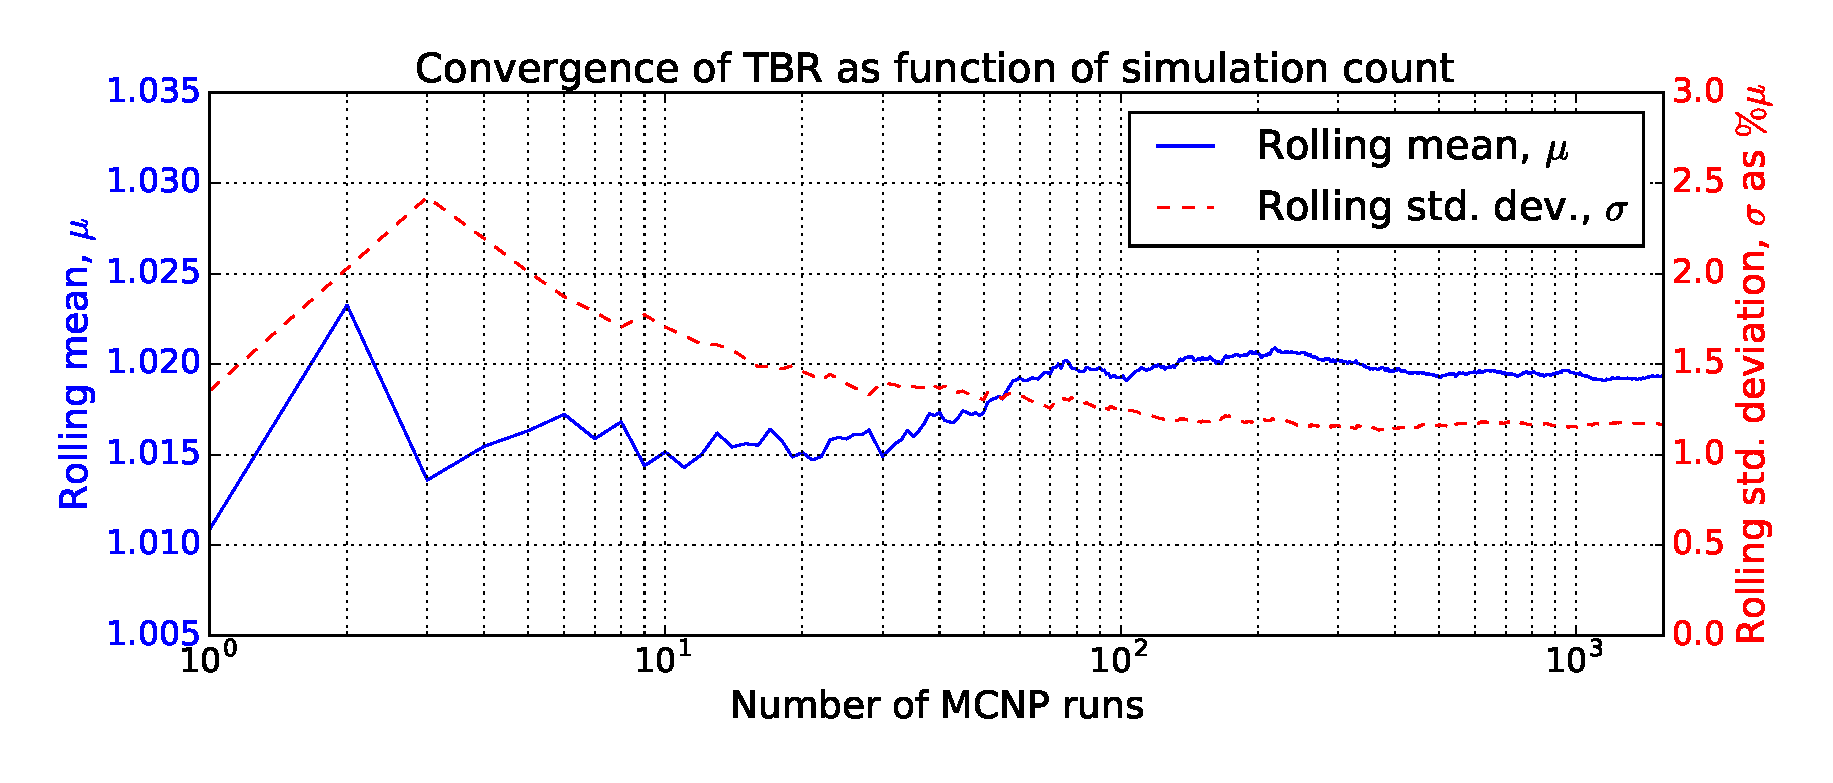
\includegraphics[width=0.8\textwidth]{hcll_convergence_1559}
	\caption[Convergence of TBR distribution as a function of simulation count.]{The simple mean and standard deviation of the TBR results is presented as a function of the number of simulations.}
	\label{fig:convergence}
\end{figure}

The TMC simulation can be seen to converge in figure~\ref{fig:convergence} at approximately 400 MCNP runs. $\mu(400) \approx 1.02$ and $\sigma(400) \approx 1.14$. The mean TBR value is 1.0193 whilst the median is 1.0200, with a one sigma standard deviation of 0.012 or 1.164\% of the mean value. 

The TBR distribution is shown as figure~\ref{fig:tbr_distribution}. Any results greater than 6$\sigma$ from the mean TBR were deemed false and discarded before analysis. This filter rejected one simulation result, where the sampled TBR value was exceptionally far from the mean value: $0.826 \approx \mu - 15\sigma$. This simulation used an erroneous \textsuperscript{207}Pb ACE file, created with unrealistic parameters. 

The shape of the distribution appears somewhat Gaussian (see equation~\ref{eq:normal}) although with an extended low-value tail. The Shapiro-Wilk test was employed to test if the TBR population have indeed been sampled from a normal distribution \cite{Shapiro1965}. Formally, a null hypothesis, $H_{0}$, that the underlying distribution is normally distributed was proposed and rejected as the computed p-value for this sample was 0.003, less than the conventional threshold for acceptance (known as $\alpha$) of 0.05\footnote{$\alpha = 0.05$ implies there is a 5\% chance the null hypothesis is incorrectly rejected and is a common value for this statistical test.}.

The disitribution is fitted well with the addition of a skewness parameter, $\gamma$ to give the `skew-normal distribution' as per equation~\ref{eq:skewed_normal}. 

\begin{equation}
  \label{eq:normal}
  f(x) = \frac{1}{\omega \sqrt{2 \pi}} e^{-\frac{(x-\xi)^{2}}{2 \omega^{2}}}
\end{equation}

\begin{equation}
  \label{eq:skewed_normal}
  g(x) = f(x) \left[1 + \mathrm{erf} \left( \frac{\gamma(x - \xi)}{\omega \sqrt{2}} \right) \right]
\end{equation}

Equation~\ref{eq:skewed_normal} is the fit function plotted in figure~\ref{fig:tbr_distribution}. $\xi$ is the location parameter, $\omega$ the shape and $\gamma$ the skewness. If the data were symmetric, $\gamma = 0$. For these data, $\gamma = -1.432$, indicating the low-value TBR tail is longer than the high-value tail. 

\begin{figure}[H]
%  \figuretitle{}
  \centering
	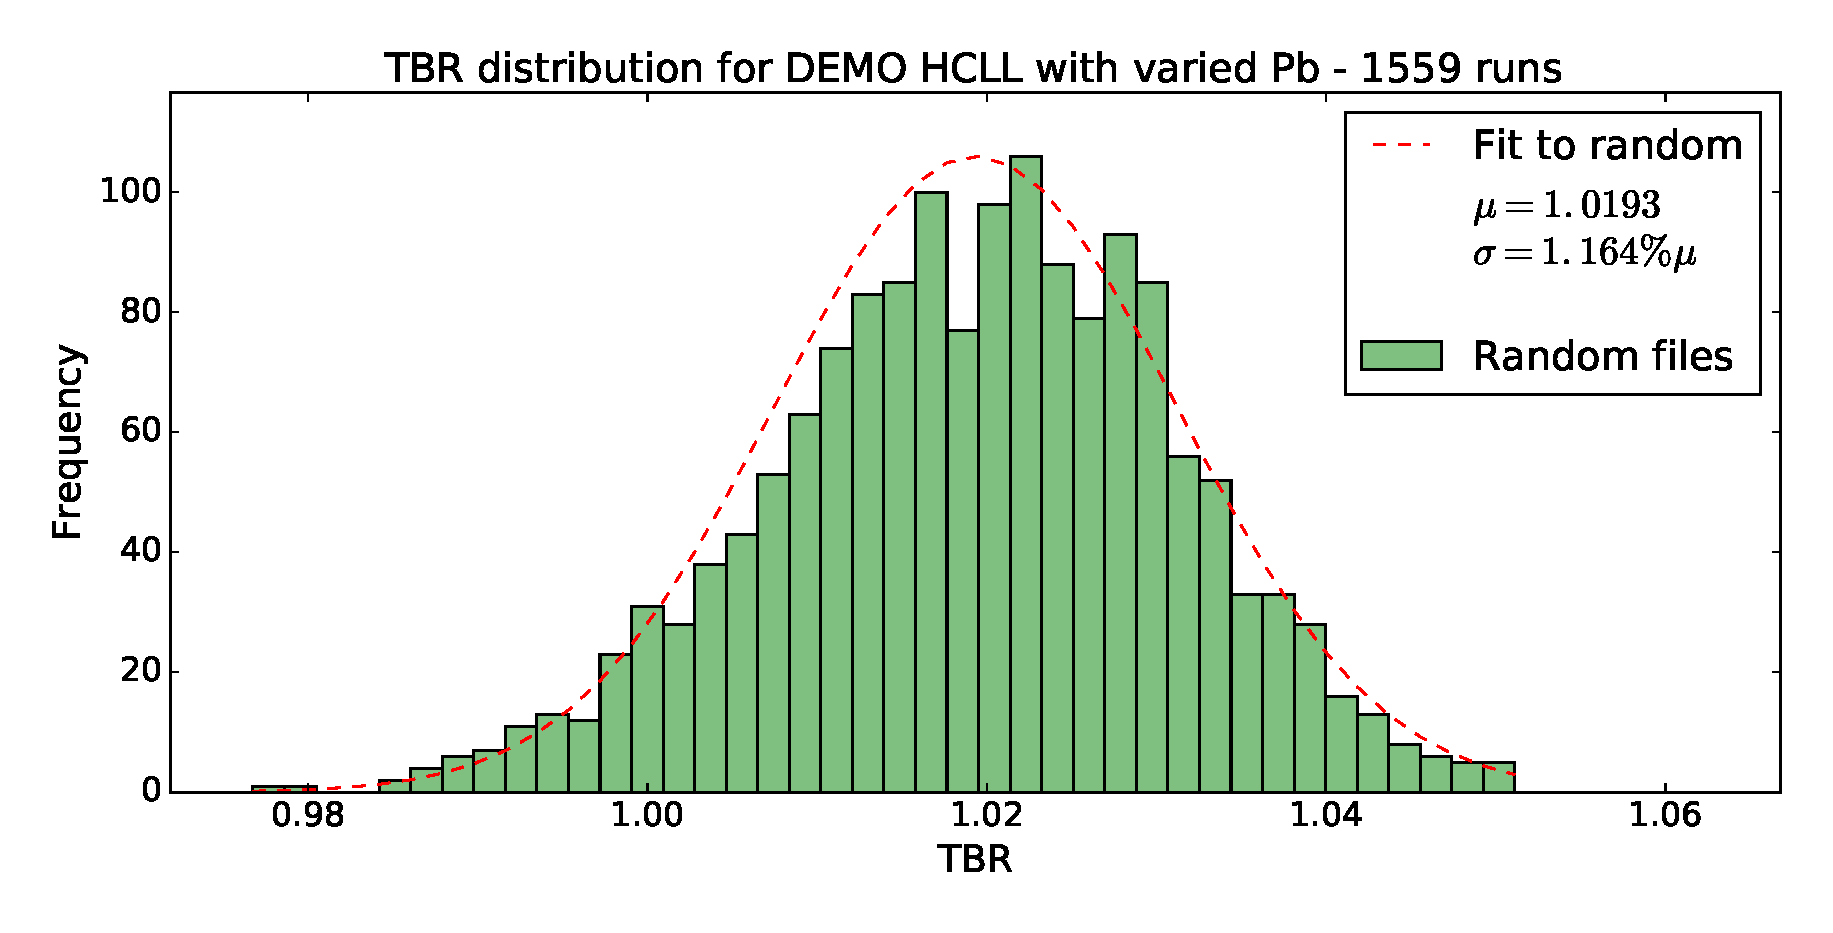
\includegraphics[width=0.8\textwidth]{hcll_hist_1559}
	\caption[DEMO HCLL TBR distribution due to lead nuclear data.]{Histogram of 1559 TBR values computed with the TMC methodology. The fit is a skew-normal distribution as described by equations~\ref{eq:normal} and \ref{eq:skewed_normal}. The standard deviation is 1.2\% of the mean value and represents the variation from TENDL2015 lead nuclear data (specifically $^{206,207,208}$Pb). Note that 5.8\% of the distribution is less than unity.}
	\label{fig:tbr_distribution}
\end{figure}

Figure~\ref{fig:tbr_n2n} shows the correlation between the n,2n cross-sections used in a given simulation and the TBR attained in that simulation. The nuclide-wise cross-sections were obtained with the Inter utility for a reaction energy of 14 MeV. As the cross-sections for each of the three lead isotopes were varied in every simulation, so the cross-sections plotted here are the elemental average values, that is, weighted by the natural abundance of each Pb isotope. A linear least squares fit has been applied to the data shown in figure~\ref{fig:tbr_n2n} and the resulting relationship plotted in blue. As the cross-section for neutron multiplying reactions of the form $^{A}$Pb(n,2n)$^{A-1}$Pb increases, so does the neutron flux available for the subsequent generation of tritium in the breeding blanket. As these reactions are endothermic, with an energy threshold relatively close to that of the D-T neutron creation energy, front loading a breeding blanket with neutron multiplying material is beneficial to TBR.

\begin{figure}[H]
%  \figuretitle{}
  \centering
	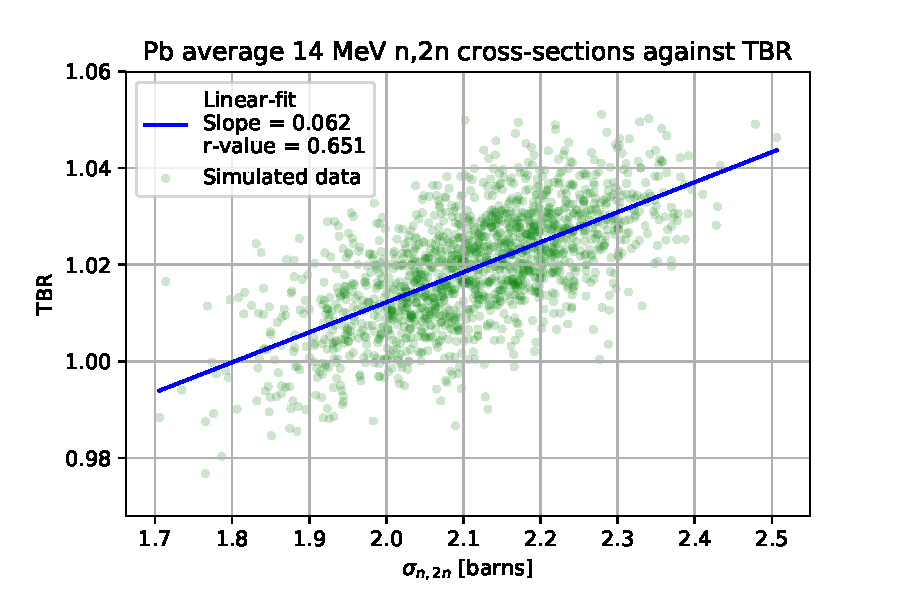
\includegraphics[width=0.7\textwidth]{TBR_n,2n}
	\caption[Correlation between $^{208}$Pb(n,2n)$^{207}$Pb cross-sections and TBR.]{Shown here are the $^{208}$Pb(n,2n)$^{207}$Pb cross-sections at 14 MeV, from the files used as input ND for the TMC simulation. They are plotted against the resulting TBR value from each simulation. There is a reasonably strong positive correlation, with increasing n,2n cross-sections resulting in an increased TBR.}
	\label{fig:tbr_n2n}
\end{figure}

The relationship between n,2n cross-section and TBR shown in figure~\ref{fig:tbr_n2n} is relatively strong, with a linear fit achieving an $r^{2}=0.43$, explaining 43\% of the total variance in TBR. Elastic scattering (shown in figure~\ref{fig:tbr_elastic}) is more weakly correlated, with a very low $r^{2}=0.02$. Figures~\ref{fig:tbr_n2n} and \ref{fig:tbr_elastic} plot relationships between the cross-section values and the simulated TBR result, but these cross-sections are only intermediate data in the TMC process. However it is possible to go one step further back and analyse for correlations between fundamental nuclear parameters and the observable of interest, TBR. 

\begin{figure}[H]
%  \figuretitle{}
  \centering
	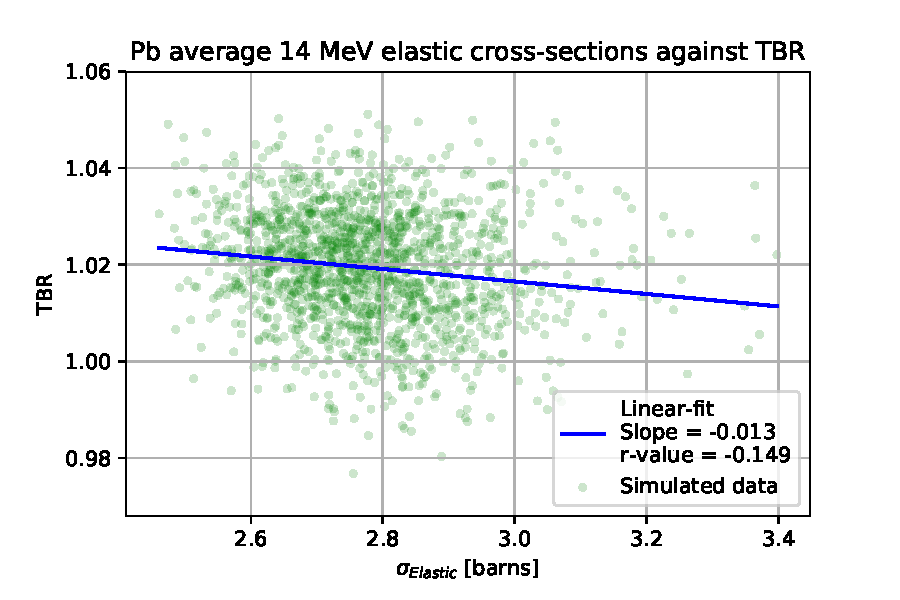
\includegraphics[width=0.7\textwidth]{TBR_Elastic}
	\caption[Correlation between $^{208}$Pb(n,el)$^{208}$Pb cross-sections and TBR.]{Shown here are the $^{208}$Pb(n,el)$^{208}$Pb cross-sections at 14 MeV, from the files used as input ND for the TMC simulation. They are plotted against the resulting TBR value from each simulation. There is a weak correlation, with a minor downward trend in TBR for increasing elastic cross-section.}
	\label{fig:tbr_elastic}
\end{figure}

The optical model is a nuclear model which aims to describe the interaction between an incident nucleon and a target nucleus. Rather than trying to solve particle behaviour \textit{ab initio}, this approach uses a complex potential energy function or simply `potential', $\mathcal{U}$ to represent nucleon-nucleus interactions. This potential energy function is a kind of description of the strong nuclear force, as a nucleon far from the nucleus, outside of the range of this force will experience no interaction. Closer, where the separation distance $r$ becomes similar to the nuclear radius $R$ and the particle may fall into the nucleus' potential well. Solving the Schr\"odinger equation with a given potential generates predictions for basic observables such as elastic scattering angular distributions and possibly the reaction and total cross-sections \cite{Hodgson1971}. 

The optical model's name is due to an analogous case where a light wave is part refracted and part absorbed in a material of complex refractive index. The imaginary part of the complex refractive index is responsible for the absorption of light. In the nuclear case, the imaginary part of the nuclear potential represents all the non-elastic behaviour. An optical model potential (OMP) contains parameters and can be fit to experimental data. In this case the optical model is known as phenomenological. In part because of the wealth of experimental nuclear physics data now available, there has been a great advance in the capabilities and generality of the optical model since its first iteration by \citeauthor{Fernbach1949} in 1949. Fits to experimental data can be global, determining parameter values which best fit a wide range of energies and nuclei, or local, where a fit is determined for a sole nucleus. These local fits produce more accurate results but clearly have worse predictive power for other situations outside of their fit parameters.

The T6 system was used to generate the TENDL2015 data used for this work. The nuclear reaction program within this suite, TALYS, employs the optical model specified by \citeauthor{Koning2003}. The potential $\mathcal{U}$ has contributions from the terms in equation~\ref{eq:talys_omp}. 

\begin{equation}
  \mathcal{U}(r,E) = - \mathcal{V}_{V}(r,E) - i\mathcal{W}_{V}(r,E) - i\mathcal{W}_{D}(r,E) + \mathcal{V}_{SO}(r,E) + i\mathcal{W}_{SO}(r,E)
  \label{eq:talys_omp}
\end{equation}

Where $\mathcal{V}_{V,SO}$ and $\mathcal{W}_{V,D,SO}$ are the real and imaginary components of the volume (V), surface (D), and spin-orbit (SO) potentials respectively. Each of these terms is separated into an energy dependent well-depth and an energy-independent radius dependent component\footnote{See §4.1.1 in \cite{TALYS2017} for more detail}. The general form of the radius dependent part for all the potentials is a Woods-Saxon shape \cite{Woods1954} as shown in equation~\ref{eq:woods-saxon}.

\begin{equation}
  \label{eq:woods-saxon}
  f(r,R,a) = \left(1 + e^{\frac{r-R}{a}}\right)^{-1}
\end{equation}

Where $r$ is the separation, $a$ a `diffuseness' parameter and $R$ the nuclear radius. $r_{V}$ is equivalent to the nuclear radius parameter $R$ in equation~\ref{eq:woods-saxon} for the $\mathcal{V}_{V}$ and $\mathcal{W}_{V}$ terms of the OMP shown as equation~\ref{eq:talys_omp}. The distribution of $r_{V}$ values that were sampled in the creation of $^{207}$Pb data for this study is shown as figure~\ref{fig:pb207_rvadjust_hist}. It is uni-modal, non-normally distributed and positively skewed. 

\begin{figure}[H]
%  \figuretitle{}
  \centering
	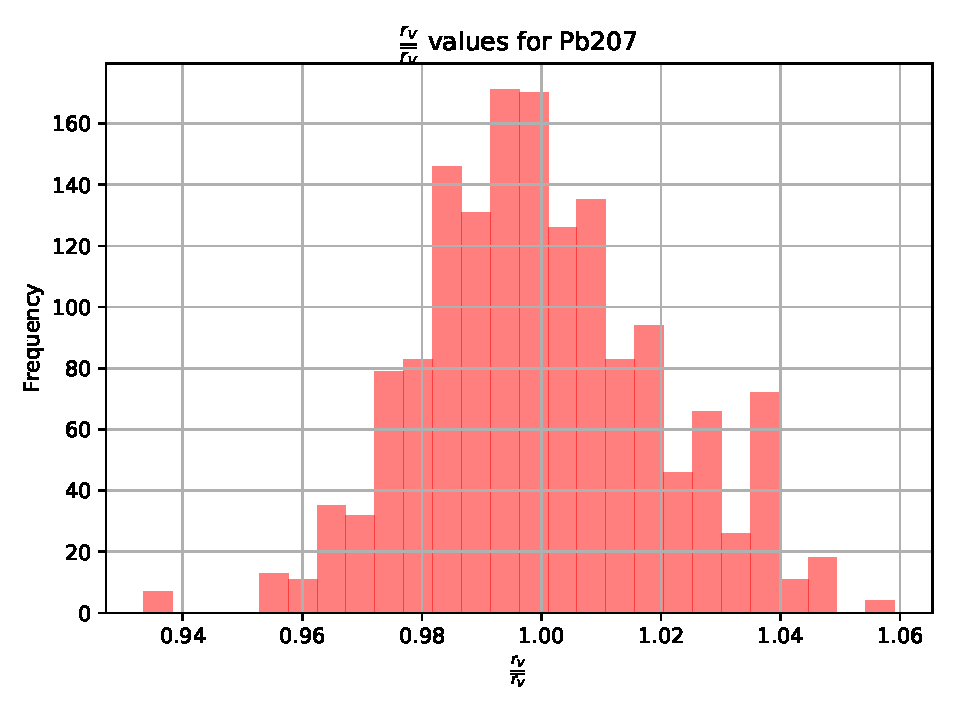
\includegraphics[width=0.8\textwidth]{rvadjust_param_Pb207_histogram}
	\caption[$r_{V}$ nuclear parameter distribution for $^{207}$Pb.]{This figure shows the distribution of nuclear radius, or $r_{V}$ values sampled in the creation of $^{207}$Pb cross-section data for this TMC work. $r_{V}$ is a geometry parameter in optical model potentials. The distribution is slightly positively skewed. The data here have been normalised by their mean to centre the distribution on unity and allow for easier comparison between parameters of different scale.}
	\label{fig:pb207_rvadjust_hist}
\end{figure}

Shown as figure~\ref{fig:pb207_rvadjust} is the relationship between $r_{V}$ as shown in figure~\ref{fig:pb207_rvadjust_hist}, as applied to the generation of \textsuperscript{207}Pb data, to the resulting TBR values. The data in figure~\ref{fig:pb207_rvadjust} have a weak relationship. A linear least squares fit is shown, with a positive slope of $m=0.06$. The $r^{2}$ value is very low at 0.01. This implies, as can be seen visually, that a great deal of variance in the data is left unexplained by the fit. However, this study has varied several nuclear parameters and nuclides simultaneously--were fewer inputs varied the relationship shown in figure~\ref{fig:pb207_rvadjust} might be clearer. 

\begin{figure}[H]
%  \figuretitle{}
  \centering
	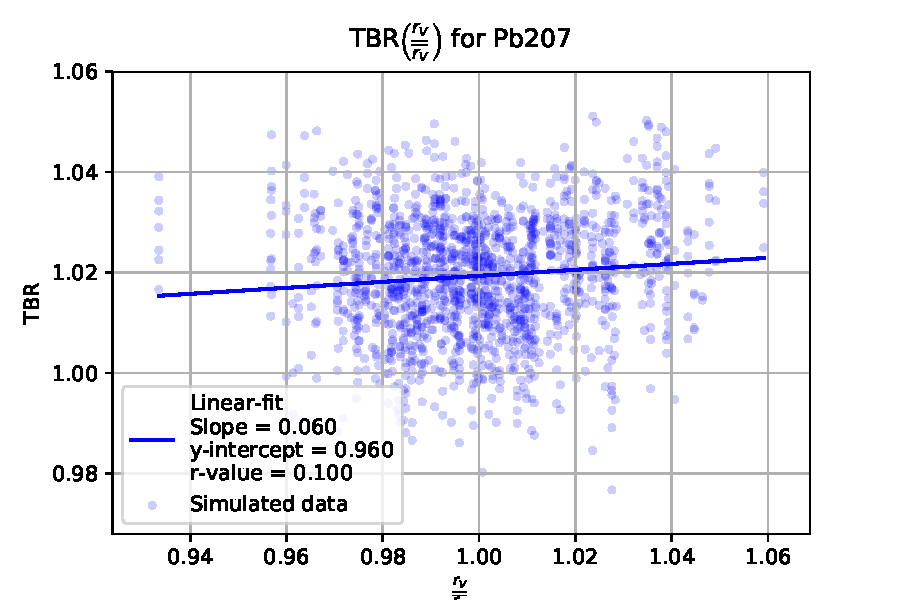
\includegraphics[width=0.7\textwidth]{Pb207_rvadjust}
	\caption[TBR as a function of $r_{V}$ for $^{207}$Pb.]{Scatter plot of the $r_{V}$ nuclear radius parameter against simulated TBR. The $r_{V}$ values have been normalised to the mean of their distribution, centring the distribution on unity. The data has been fit with a linear relationship, with the fit data shown in the plot. A minor positive correlation is registered.}
	\label{fig:pb207_rvadjust}
\end{figure}

Performing a least-squares fit on all the varied nuclear parameters against the simulated TBR results, we can estimate which parameters TBR is most sensitive to. One could take the slope of the linear best fit line as the sensitivity, however as many of the correlations here are very poor, the slope $m$ is multiplied by the $r^{2}$ value of the fit, to handicap parameters with worse fits to TBR data. For \textsuperscript{207}Pb the parameter correlation bar chart is shown as figure~\ref{fig:pb207_param_correl}, with the ordinate displaying the $m \cdot r^{2}$ of the fit line. Prior to fitting, the parameters were normalised to their mean value so their absolute values do not bias the resulting line gradients. It can be seen that the sampled variation in the $r_{V}$ parameter for \textsuperscript{207}Pb results in the most change in simulated TBRs. The gradient is positive, with an increase value of the nuclear radius $r_{V}$ resulting in a higher TBR. The most important parameter for \textsuperscript{206}Pb's contribution to TBR uncertainty is $v_{1}$, a multiplicative factor in the energy dependent part of $\mathcal{V}_{V}$, the real volume potential. This relationship is an inverse one, with an increase in $v_{1}$ weakly correlated with a decrease in TBR. $^{208}$Pb is most affected by $d_{1}$, a multiplicative parameter in the energy dependent component of $\mathcal{W}_{D}$, the imaginary surface potential. Better constraining these parameters might act to reduce uncertainty in future lead based blanket analyses. This could be achieved with more experimental data or advances in model theory.

% Pb208 = d1, Pb206 = v1 and Pb207 = rv are most important parameters

\begin{figure}[H]
%  \figuretitle{}
  \centering
	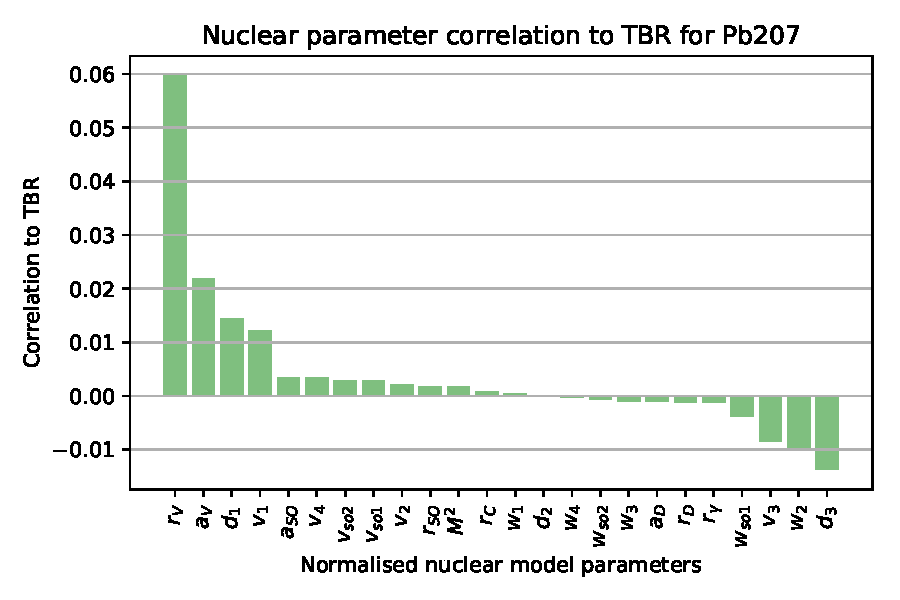
\includegraphics[width=0.8\textwidth]{Pb207_param_correl}
	\caption[Strength of correlation between $^{207}$Pb nuclear parameters and TBR.]{This bar chart shows the relationship between various nuclear parameters and TBR simulation data. The abscissa shows a variety of model parameters, the vast majority from optical model potentials. The ordinate values for each parameter are measures of the correlation between sampled parameter data and the TBR. The correlation measure is the slope multiplied by r-squared value of a linear fit to each dataset, the latter acting to relegate parameters which explain very little of the TBR variance. The parameter data was normalised to its mean before fitting, so that parameter absolute values did not bias the results. The majority of parameters studied have little correlation with TBR, leaving a few optical model parameters such as $r_{V}$ and $d_{1}$.}
	\label{fig:pb207_param_correl}
\end{figure}

% \begin{figure}[H]
% %  \figuretitle{}
%   \centering
%   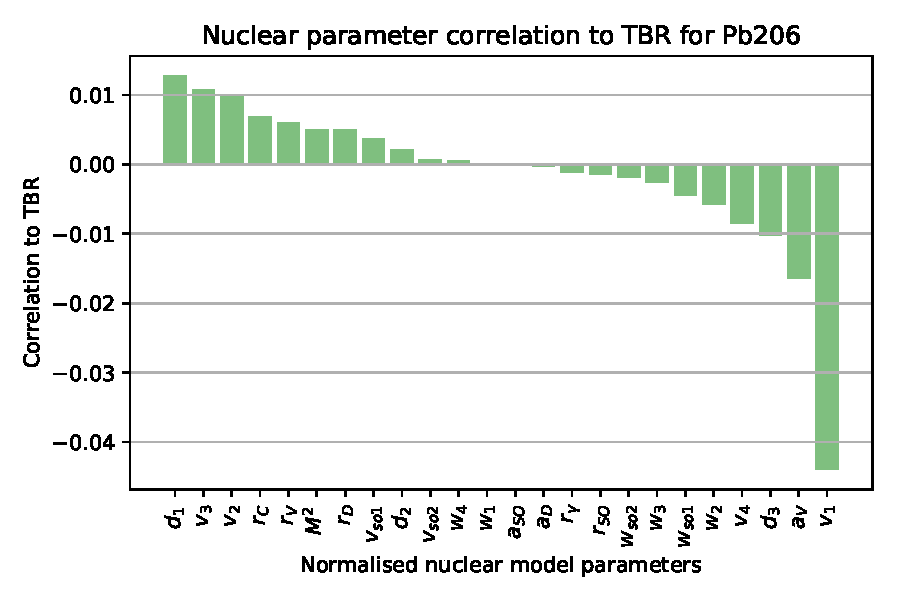
\includegraphics[width=0.8\textwidth]{Pb206_param_correl}
%   \caption{}
%   \label{fig:pb206_param_correl}
% \end{figure}
%
% \begin{figure}[H]
% %  \figuretitle{}
%   \centering
%   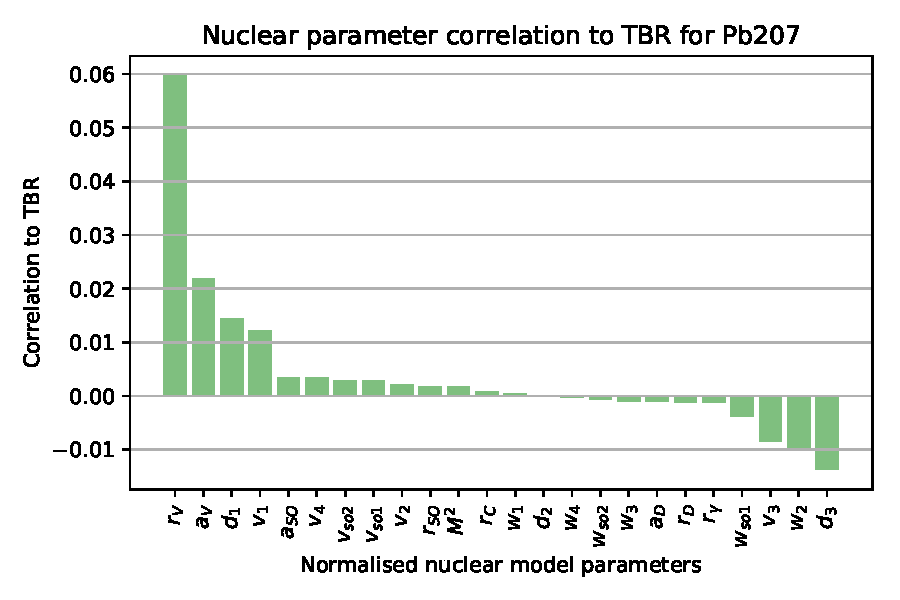
\includegraphics[width=0.8\textwidth]{Pb207_param_correl}
%   \caption{}
%   \label{fig:pb207_param_correl}
% \end{figure}

%%%%% WARNING ---->
% Even energy dependent adjustment of the geometry is possible as a last resort to fit data, using the rvadjustF, etc. keywords.
% Have we found a strong correlation between a fudge parameter and the TBR? Oh dear

\section{Conclusion}
TBR uncertainty has been computed with the TMC technique, investigating the contribution of uncertain nuclear data from the three major lead isotopes. The standard deviation is 1.2\% of the mean TBR. However, note that 5.8\% of the distribution is less than unity. While the average value may appear to be feasible, it should be stressed that there is a non-negligible probability of a value below a required limit. The TBR values are relatively low as this particular model has not been optimised for TBR and any practical design should have a TBR $\approx 1.1$ \cite{Fischer2015}, but in future design studies engineers should be aware of the probability of non-compliant operational parameters. 

The TENDL-2015 nuclear data investigated in section \ref{subsec:data}, which is not necessarily Gaussian in shape, has yielded a TBR distribution with a small but finite negative skewness, an extended low-value tail. Decreasing the uncertainty in the aforementioned important optical model parameters, $v_{1}$ for \textsuperscript{206}Pb, $r_{V}$ for \textsuperscript{207}Pb and $d_{1}$ for \textsuperscript{208}Pb, would potentially act to reduce the uncertainty in future TBR analyses.

Uncertainty propagation in Monte-Carlo type radiation transport problems has often previously been computed using linear perturbation theory approaches. Unfortunately these are only applicable for small changes in the input data. They are also unable to reproduce probability distributions of the integral quantity of interest \cite{Rising2012}. Whilst figure \ref{fig:tbr_distribution} shows a TBR distribution that is only slightly skewed, that is not to say other fusion quantities will not be. Koning \& Rochman have demonstrated that fast and accelerator driven fission systems can have significantly skewed $k_{\mathrm{eff}}$ values, well described by an Extreme Value Fit (EVD) \cite{Koning2008}.

Future work on TBR in HCLL could include the effect of other nuclides and elements which TBR is sensitive to including iron and oxygen as well as a completely correlated uncertainty propagation method employing lithium if data for light nuclides becomes available.

More generally, when solving for integral quantities in nuclear fusion systems, thought should be given to fully-correlated uncertainty propagation and the form of the resulting probability distributions. In particular, whether a non-normal distribution with increased likelihood of extreme behaviour would have engineering design or safety implications for TBR, nuclear heating, fast flux, gas production or damage terms. Moreover, in all analyses for design applications the non-negligible probability of operational parameters in unacceptable regimes should be borne in mind.

